\documentclass[11pt]{article}
\input{glyphtounicode}
\pdfgentounicode=1
\usepackage[utf8]{inputenc}
\usepackage[T1]{fontenc}
\usepackage{lmodern}
\usepackage{amsmath,amssymb,amsthm}
\numberwithin{equation}{section}
\usepackage[margin=1.05in]{geometry}
\usepackage{booktabs}
\usepackage{array}
\usepackage{longtable}
\usepackage{graphicx}
\usepackage{float}
\usepackage[section]{placeins}
\usepackage{natbib}
\bibliographystyle{apalike}
\usepackage{caption}
\captionsetup{font=small}
\usepackage{xcolor}
\definecolor{linkblue}{RGB}{20,70,140}
\PassOptionsToPackage{hyphens}{url}
\usepackage{xr-hyper}
\usepackage[colorlinks=true,linkcolor=linkblue,citecolor=linkblue,urlcolor=linkblue]{hyperref}
\hypersetup{pdftitle={Online Appendix: Before the Labor Market or Inside It? Family Background, Earnings Dynamics, and the Return to College},pdfauthor={Jiachen Jin}}
\usepackage{setspace}
\setstretch{1.15}
\emergencystretch=1.5em
\newcolumntype{L}[1]{>{\raggedright\arraybackslash}p{#1}}

% ---------------------------------------------------------------------------
% The one place to set the address of the public repository.
\newcommand{\repourl}{https://github.com/JiachenJin1001/family-background-earnings-china}
% ---------------------------------------------------------------------------
\newcommand{\code}[1]{\href{\repourl/blob/main/#1}{\nolinkurl{#1}}}
\newcommand{\folder}[1]{\href{\repourl/tree/main/#1}{\nolinkurl{#1}}}
\makeatletter\g@addto@macro{\UrlBreaks}{\do\/\do\_\do\.}\makeatother
\newcommand{\paperpdf}{\href{\repourl/blob/main/unified/paper/main.pdf}{the paper}}
\newcommand{\pinc}{\overline{\mathrm{ParentInc}}}

% cross-references into the paper (labels carry the prefix P-)
\IfFileExists{../paper/main.aux}{\externaldocument[P-]{../paper/main}}{%
\IfFileExists{../unified/paper/main.aux}{\externaldocument[P-]{../unified/paper/main}}{%
\externaldocument[P-]{paper_main}}}

% part2_macros.tex
% Definitions needed by part2_formal_results.tex. \input this file in the
% preamble of the host document, after amsmath is loaded or not (the two
% packages below are requested here in either case).
%
% Every definition is guarded, so the host document may define the same
% command or theorem environment before this file is read.
%
% Numbering: the theorem-like environments are numbered within section.
% part2_formal_results.tex also expects equations and tables to be numbered
% within section; the host document sets that with
%   \numberwithin{equation}{section}  and  \numberwithin{table}{section}.

\RequirePackage{amsmath,amssymb}
\RequirePackage{amsthm}

\providecommand{\E}{\mathrm{E}}
\providecommand{\Var}{\mathrm{Var}}
\providecommand{\Cov}{\mathrm{Cov}}
\providecommand{\Corr}{\mathrm{Corr}}
\providecommand{\plim}{\operatorname{plim}}
\providecommand{\Direct}{\mathrm{Direct}}

\makeatletter
\theoremstyle{plain}
\@ifundefined{proposition}{\newtheorem{proposition}{Proposition}[section]}{}
\@ifundefined{corollary}{\newtheorem{corollary}[proposition]{Corollary}}{}
\@ifundefined{lemma}{\newtheorem{lemma}[proposition]{Lemma}}{}
\theoremstyle{definition}
\@ifundefined{assumption}{\newtheorem{assumption}{Assumption}[section]}{}
\theoremstyle{remark}
\@ifundefined{remark}{\newtheorem{remark}[proposition]{Remark}}{}
\theoremstyle{plain}
\makeatother

% links to files of the repository (the host document defines \code with a hyperlink)
\providecommand{\code}[1]{\texttt{\detokenize{#1}}}


\renewcommand{\thesection}{\Alph{section}}
\renewcommand{\thesubsection}{\Alph{section}.\arabic{subsection}}
\renewcommand{\thetable}{A\arabic{table}}
\renewcommand{\thefigure}{A\arabic{figure}}

\title{Online Appendix\\[6pt]
{\large\emph{Before the Labor Market or Inside It?\\[-6pt] Family Background, Earnings Dynamics, and the Return to College}}}
\author{Jiachen Jin\thanks{New York University,
\texttt{jj4608@stern.nyu.edu}. Tables, figures, sections and equations
of the paper are cited as ``Table~\ref{P-tab:md} of the paper''; objects
numbered A1, A2, \ldots\ belong to this appendix. Every link in blue
opens the file it names in the public repository.}}
\date{October 2026}

\begin{document}
\maketitle
\thispagestyle{empty}

\noindent This appendix has three parts. Part I reports supplementary
results in the order of the paper: the data, the earnings process, the
attenuation schedule, the premium, the expansion design, and the
decomposition. Part II states and proves the formal results the paper
uses. Part III is a guide to the replication files: which script
produces each table and figure, how to run the pipeline, and how to
obtain the data. Every table in Part I is written by a script from the estimation output, and the repository carries the
checks that compare every number printed in \paperpdf\ and in this appendix with that output.

\begin{table}[H]
\centering
\small
\caption{Where to find the material behind each section of the paper.}
\label{oatab:map}
\begin{tabular}{@{}L{5.4cm}L{5.6cm}L{4.0cm}@{}}
\toprule
Section of the paper & Supplementary results & Formal results \\
\midrule
\ref{P-sec:data}. Data & Section~\ref{oa:data} & \\
\ref{P-sec:process}. The earnings process and family background &
Section~\ref{oa:process} & Part II, minimum-distance estimator \\
\ref{P-sec:measurement}. What the process implies for measurement &
Section~\ref{oa:measurement} & Part II, attenuation schedule \\
\ref{P-sec:premium}. The level premium & Section~\ref{oa:premium} & \\
\ref{P-sec:expansion}. The college channel: the 1999 expansion &
Section~\ref{oa:expansion} & \\
\ref{P-sec:mediation}. Decomposing the premium &
Section~\ref{oa:decomposition} & Part II, content of the direct term \\
\bottomrule
\end{tabular}
\end{table}

\clearpage
\tableofcontents
\newpage

\part*{Part I. Supplementary results}
\addcontentsline{toc}{part}{Part I. Supplementary results}

\section{Data and sample}
\label{oa:data}

\subsection{Income variables by wave}

The survey's measure of personal labor income changed definition in 2014
(Section~\ref{P-sec:income} of the paper). Table~\ref{oatab:income}
lists the variable used in each wave. The earnings outcomes of the
paper use the waves in which the variable covers jobs only, 2014 to
2022. For the two estimates that use a seven-wave
panel, a measure that covers jobs only is reconstructed for 2010 and
2012 from the components that the questionnaire records. For 2010 these
are the monthly wage of the main job (annualized), the annual bonus,
self-employment income, and income from secondary jobs; for 2012, the
annual after-tax income of each job, the net income of each business,
income from part-time work, and income from work for other agricultural
households. Among all respondents aged 22 to 55 with positive income, the variance of log income under the survey's own variable of Table~\ref{oatab:income} is 2.26 in the 2010 wave and 1.37 in the 2012 wave, against 0.87, 1.04, 0.85, 0.93, and 0.98 in the five waves from 2014 to 2022 (\code{unified/code/u17_income_variance_by_wave.py}).

\begin{table}[H]
\centering
\small
\caption{The CFPS income variable used in each wave.}
\label{oatab:income}
\begin{tabular}{@{}lll@{}}
\toprule
Wave & Variable & Concept \\
\midrule
2010 & \texttt{income} & jobs, transfers and asset income together \\
2012 & \texttt{income\_adj} & jobs, transfers and asset income together \\
2014, 2016, 2018 & \texttt{income} & jobs only \\
2020, 2022 & \texttt{emp\_income} & jobs only \\
\bottomrule
\end{tabular}
\end{table}

\subsection{Sample screens by family background}

Table~\ref{oatab:screens} follows children with a valid retrospective
report of parental occupation through the screens of
Section~\ref{P-sec:sample} of the paper. The screens pass advantaged
and less advantaged children at nearly the same rate, so selection into the sample is unlikely to account for the difference between the two groups. Before
any earnings screen, positive labor income appears in
55.6 percent of the person-waves of advantaged and 49.7 percent of the person-waves of less advantaged children%
 at ages 22 to 55.

\begin{table}[H]
\centering
\small
\caption{Sample screens by family background.}
\label{oatab:screens}
\setlength{\tabcolsep}{4pt}
\begin{tabular}{@{}p{6.0cm}cccc@{}}
\toprule
 & \multicolumn{2}{c}{Children} & \multicolumn{2}{c}{Percent of first row} \\
\cmidrule(lr){2-3}\cmidrule(lr){4-5}
Screen & Advantaged & Less advantaged & Advantaged & Less advantaged \\
\midrule
Retrospective report, family income of the parental household, observed at ages 22--55 in a 2014--2022 wave & 1,661 & 9,013 & 100.0 & 100.0 \\
Trimming and at least two waves of positive labor income at ages 22--55 (the sample of the paper) & 755 & 3,781 & 45.5 & 42.0 \\
Of these, at least three waves (Sections 3 and 4 of the paper) & 420 & 2,103 & 25.3 & 23.3 \\
Of the sample, at least two waves at ages 30 and over (level of earnings, Sections 5 to 7 of the paper) & 453 & 2,321 & 27.3 & 25.8 \\
\bottomrule
\end{tabular}

\par\smallskip
\begin{minipage}{0.92\textwidth}
\footnotesize\emph{Notes:} Advantaged children have at least one
parent in an official, managerial, or professional occupation (CSCO
major group 1 or 2) when the child was fourteen; less advantaged children are
all others. Source: \code{unified/code/u14_sample_facts.py}.
\end{minipage}
\end{table}

\subsection{Variable definitions}

\begin{table}[H]
\centering
\small
\caption{Main variables.}
\label{oatab:vars}
\begin{tabular}{@{}L{3.6cm}L{11.0cm}@{}}
\toprule
Variable & Definition \\
\midrule
$H_i$ & Equal to one if either parent held an occupation in CSCO major
group 1 or 2 when the child was fourteen; retrospective reports from the
2012, 2020 and 2022 waves. \\
$M_i$ & Sixteen or more completed years of schooling (a four-year
college degree). \\
$\bar y_{io}$, $\bar y_{ib}$ & Mean of log annual labor income, net of
survey-year effects, over a child's waves at ages 30 and over (the
level of earnings; at least two such waves) and over the waves at ages
22 to 29, among the 2014 to 2022 waves with positive income; incomes
below 1,000 yuan and the top 1 percent within each wave are dropped. \\
$\pinc_i$ & Mean of log family income of the parental household across
all observed waves; a second version uses the linked parents' own labor
income. \\
$Z_{i}$ & Provincial intensity of the expansion multiplied by the
exposure ratio of the child's birth cohort; the province and the birth year are those recorded in the first wave in which the child is observed at ages 22 to 55. \\
Professional occupation & The child's own occupation in CSCO major
group 1 or 2; the outcome of the paper is the share of the child's
waves at ages 30 and over in such an occupation. \\
Controls of the expansion design & $H_i$, $\pinc_i$, gender, urban
residence, province effects, one indicator per birth year, an indicator
for the row at 30 and over, and its product with $H_i$. \\
\bottomrule
\end{tabular}
\end{table}

\section{The earnings process}
\label{oa:process}

\subsection{Variances and first-order autocovariances by wave}
\label{oa:autocov}

Figure~\ref{P-fig:autocov} of the paper plots the variances of residual
log earnings in each wave and the autocovariances by lag for the two
groups. Table~\ref{oatab:autocov} gives the variances and the
first-order autocovariances behind it, with their bootstrap standard
errors.

\begin{table}[H]
\centering
\small
\caption{Empirical autocovariances of residual log earnings, pooled and by group.}
\label{oatab:autocov}
\begin{tabular}{@{}lccccc@{}}
\toprule
& \multicolumn{5}{c}{Variances} \\
\cmidrule(lr){2-6}
& 2014 & 2016 & 2018 & 2020 & 2022 \\
\midrule
Pooled & 0.49 (0.02) & 0.58 (0.04) & 0.42 (0.02) & 0.46 (0.02) & 0.41 (0.02) \\
Advantaged & 0.47 (0.06) & 0.49 (0.09) & 0.40 (0.04) & 0.44 (0.04) & 0.43 (0.05) \\
Less advantaged & 0.50 (0.03) & 0.60 (0.03) & 0.43 (0.02) & 0.46 (0.02) & 0.40 (0.02) \\
\midrule
& \multicolumn{5}{c}{First-order autocovariances} \\
\cmidrule(lr){2-6}
& 2014, 2016 & 2016, 2018 & 2018, 2020 & 2020, 2022 & \\
\midrule
Pooled & 0.11 (0.04) & 0.15 (0.02) & 0.18 (0.01) & 0.19 (0.01) & \\
Advantaged & 0.21 (0.14) & 0.15 (0.04) & 0.17 (0.02) & 0.24 (0.04) & \\
Less advantaged & 0.10 (0.03) & 0.15 (0.02) & 0.18 (0.01) & 0.18 (0.01) & \\
\bottomrule
\end{tabular}

\par\smallskip
\begin{minipage}{0.9\textwidth}
\footnotesize\emph{Notes:} Children with at least three waves of earnings, 2014 to 2022 panel; residuals demeaned within group and year. Bootstrap standard errors in parentheses (200 replications that resample children). Across all fifteen pairwise moments, including the higher lags not displayed, no gap between the two groups exceeds two standard errors; the largest standardized gap is 1.58, at the (2014,\,2022) covariance%
. Source:
\code{income_dynamics/code/m5_md_weighted_and_ridge.py}.
\end{minipage}
\end{table}

\subsection{Joint test of moment equality}
\label{oa:jointtest}

Section~\ref{P-sec:md} of the paper reports that a joint test does not
reject equality of the fifteen variances and autocovariances of the two
groups. The test takes the vector of fifteen gaps between advantaged
and less advantaged children in the moments of the 2014 to 2022 panel
(residuals demeaned within group and year), estimates its covariance
from a bootstrap that resamples children within each group, and computes the quadratic form of the gaps in the inverse of that covariance.
The statistic is 17.0 on fifteen degrees of freedom ($p = 0.32$); a bootstrap-calibrated version that compares the statistic with the distribution of centered bootstrap draws gives $p = 0.311$ with 2,000 draws%
. Source:
\code{income_dynamics/code/m16_joint_moment_test.py}.

\subsection{What the design could have detected}

\begin{table}[H]
\centering
\small
\caption{Minimum detectable differences between the two groups.}
\label{oatab:mde}
\begin{tabular}{@{}lccc@{}}
\toprule
 & Gap, advantaged minus & Standard & Minimum detectable \\
Parameter & less advantaged children & error & difference \\
\midrule
Permanent variance & $-$0.046 & 0.030 & 0.08 \\
Variance of transitory shocks & $-$0.011 & 0.028 & 0.08 \\
Transitory persistence & 0.212 & 0.084 & 0.24 \\
Permanent share & $-$0.092 & 0.068 & 0.19 \\
Arellano--Bond persistence interaction & --- & 0.094 & 0.26 \\
\bottomrule
\end{tabular}

\par\smallskip
\begin{minipage}{0.92\textwidth}
\footnotesize\emph{Notes:} Standard errors of the gaps from the
bootstrap of Table~\ref{P-tab:md} of the paper; the last row uses the
two-step sandwich standard error of the interaction in
Table~\ref{P-tab:ab} of the paper. The minimum detectable difference at
80 percent power and the 5 percent level is 2.8 times the standard
error. Source: \code{income_dynamics/code/m13_mde_group_null.py}.
\end{minipage}
\end{table}

\subsection{Alternative error structures}
\label{oa:errorstructures}

The paper fits a permanent effect plus an AR(1) transitory component.
Table~\ref{oatab:criterion} reports the minimized criterion when the
transitory component is instead ARMA(1,1) or MA(1), and when the
permanent effect is replaced by a random walk. The richer transitory
structures leave the criterion where it was, and the random walk fits
worse in every sample.

\begin{table}[H]
\centering
\small
\caption{Minimized criterion under alternative error structures.}
\label{oatab:criterion}
{\setlength{\tabcolsep}{4pt}\begin{tabular}{@{}lcccc@{}}
\toprule
 & Permanent effect & Permanent effect & Permanent effect & Random-walk \\
Sample & plus AR(1) & plus ARMA(1,1) & plus MA(1) & permanent component \\
\midrule
Pooled & 29.3 & 28.9 & 29.8 & 35.3 \\
Advantaged children & 2.7 & 2.6 & 3.1 & 5.6 \\
Less advantaged children & 29.8 & 29.5 & 29.9 & 32.8 \\
\bottomrule
\end{tabular}
}
\par\smallskip
\begin{minipage}{0.92\textwidth}
\footnotesize\emph{Notes:} Minimum distance with weights equal to the number of children observed in both waves of each moment, on all fifteen variances and
autocovariances of the 2014 to 2022 panel. Criterion values are
comparable within a row. Source:
\code{unified/code/u7_error_structures.py}.
\end{minipage}
\end{table}

\subsection{Diagnostics for the dynamic-panel estimate}

Table~\ref{oatab:abdiag} reports the serial-correlation tests behind
Table~\ref{P-tab:ab} of the paper. On either panel, the test of second-order serial correlation does not reject the absence of second-order correlation on which instruments dated two waves back rely. The five-wave estimates are computed three times: in Python, in a Mata implementation that builds the same moments, and in Stata's \texttt{xtabond2} under the same collapsed instrument layout with Windmeijer-corrected standard errors. Python and Mata agree to four decimals on both coefficients, their standard errors, and the Hansen statistic; \texttt{xtabond2} gives 0.058 (SE 0.036) and 0.010 (SE 0.096) for the two coefficients of Table~\ref{P-tab:ab} of the paper, and a Hansen statistic of 2.34 against 2.38. For the system GMM row, Python and \texttt{xtabond2} give persistence of 0.109 and 0.111, and the Hansen test rejects in both (20.86 and 20.49 on four degrees of freedom). The Stata files are in \folder{income_dynamics/code/stata}, and \code{income_dynamics/output/tables/stata_abgmm_parity.csv} collects the three sets of estimates.

\begin{table}[H]
\centering
\small
\caption{Serial-correlation tests for the Arellano--Bond estimates.}
\label{oatab:abdiag}
\setlength{\tabcolsep}{4pt}
\begin{tabular}{@{}p{4.6cm}cccc@{}}
\toprule
 & Persistence, & & & Persistence, instruments \\
 & main & & & lagged three or \\
Panel & estimate (SE) & $m_1$ ($z$) & $m_2$ ($z$ [$p$]) & more waves (SE) \\
\midrule
Five waves, 2014--2022 & 0.058 (0.036) & $-$5.57 & 0.68 [0.50] & $-$0.81 (0.89) \\
Seven waves, 2010--2022 (reconstructed) & 0.062 (0.033) & $-$7.17 & $-$0.08 [0.93] & $-$0.29 (0.42) \\
\bottomrule
\end{tabular}

\par\smallskip
\begin{minipage}{0.94\textwidth}
\footnotesize\emph{Notes:} Two-step difference GMM as in
Table~\ref{P-tab:ab} of the paper. $m_1$ and $m_2$ are cluster-robust
statistics for first- and second-order serial correlation of the
differenced residuals; $m_1$ is negative by construction. The last column re-estimates with instruments dated three waves back and earlier; with persistence near 0.06, lagged levels three or more waves back carry little of the variation in the lagged difference, and the standard errors are correspondingly larger. Source:
\code{income_dynamics/code/m17_ab_diagnostics.py}.
\end{minipage}
\end{table}

\subsection{Nonlinear persistence across runs of the estimator}
\label{oa:nonlinear}

The nonlinear state equation of Section~\ref{P-sec:abb} of the paper is estimated by stochastic EM, so its estimates vary with the random draws. Table~\ref{oatab:nonlinear} sets the average persistence reported in the paper beside the mean and the range over ten further runs with different seeds. In every one of the ten runs the average persistence of advantaged children is above that of less advantaged children.

\begin{table}[H]
\centering
\small
\caption{Average nonlinear persistence: the run reported in the paper and ten further runs.}
\label{oatab:nonlinear}
\begin{tabular}{@{}lcccc@{}}
\toprule
 & Run reported & \multicolumn{3}{c}{Ten further runs} \\
\cmidrule(lr){3-5}
Children & in the paper & Mean & Smallest & Largest \\
\midrule
All children with at least three waves & 0.46 & 0.48 & 0.42 & 0.54 \\
Advantaged children & 0.54 & 0.53 & 0.52 & 0.56 \\
Less advantaged children & 0.44 & 0.45 & 0.40 & 0.49 \\
\bottomrule
\end{tabular}

\par\smallskip
\begin{minipage}{0.86\textwidth}
\footnotesize\emph{Notes:} Persistence $\partial Q(s, u)/\partial s$ averaged uniformly over a $5 \times 5$ lattice of quantiles of the state and of the shock rank, 2014 to 2022 panel. Sources: \code{income_dynamics/code/ws_05b_abb_stochastic_em.py} (the run reported in the paper) and \code{unified/code/u15_nonlinear_persistence_runs.py} (ten runs).
\end{minipage}
\end{table}

\section{Attenuation: the schedule, rank-rank slopes, and the linked parents}
\label{oa:measurement}

Figure~\ref{oafig:attenuation} plots the schedule of
Table~\ref{P-tab:eta} of the paper out to ten waves. Part II derives
the exact schedule, gives the closed form for the number of waves
needed to reach a target, and reports bootstrap intervals.

\begin{figure}[H]
\centering
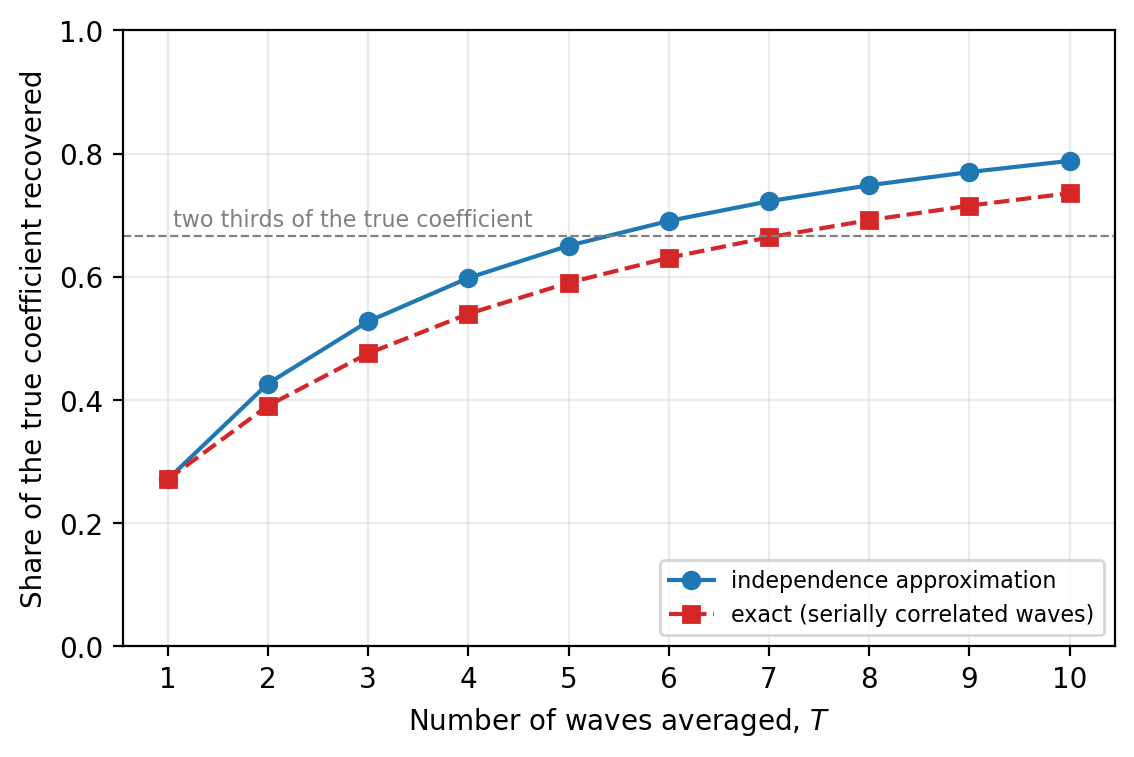
\includegraphics[width=0.68\textwidth]{figures/oa_attenuation.png}
\caption{Share of the coefficient on permanent income recovered by an
average of $T$ waves, at the pooled estimates of
Table~\ref{P-tab:md} of the paper.}
\label{oafig:attenuation}
\end{figure}

\subsection{Rank-rank slopes}

\begin{table}[H]
\centering
\small
\caption{Attenuation of rank-rank slopes by number of waves averaged
(simulation from the fitted process).}
\label{oatab:rank}
\begin{tabular}{@{}cccc@{}}
\toprule
Waves & Share recovered, & Rank-rank slope, child's rank & Rank-rank slope, child's rank \\
averaged & levels (exact) & from permanent income & from three waves \\
\midrule
1 & 0.27 & 0.52 & 0.36 \\
2 & 0.39 & 0.62 & 0.43 \\
3 & 0.48 & 0.68 & 0.47 \\
4 & 0.54 & 0.73 & 0.51 \\
5 & 0.59 & 0.77 & 0.53 \\
6 & 0.63 & 0.79 & 0.55 \\
7 & 0.66 & 0.81 & 0.56 \\
\bottomrule
\end{tabular}

\par\smallskip
\begin{minipage}{0.92\textwidth}
\footnotesize\emph{Notes:} The rank-rank columns give the ratio of the
slope under a $T$-wave measure of parental income to the slope under
permanent income. The last column also measures the child's rank from
three waves. Part II gives a closed form under normality that
reproduces the third column to within 0.004. Source:
\code{income_dynamics/code/m8_rank_attenuation_sim.py}.
\end{minipage}
\end{table}

\subsection{The earnings process of linked parents}

\begin{table}[H]
\centering
\small
\caption{The earnings process of linked working parents.}
\label{oatab:parent}
\begin{tabular}{@{}lc@{}}
\toprule
Quantity & Value \\
\midrule
Parents (person-waves) & 542 (1,878) \\
Variance of residual log earnings & 0.690 \\
First-order autocovariance & 0.301 \\
Autocovariance at longer lags & 0.294 \\
Permanent share & 0.43 [0.35, 0.49] \\
Transitory persistence & 0.02 \\
\bottomrule
\end{tabular}

\par\smallskip
\begin{minipage}{0.9\textwidth}
\footnotesize\emph{Notes:} Linked parents aged sixty or younger with
three or more waves of positive labor income over 2014 to 2022; log income is residualized as for the children. The permanent share is
the autocovariance at longer lags relative to the variance; the
interval is from a bootstrap that resamples parents. This is the parents' earnings process used in the second row of panel B of
Table~\ref{P-tab:eta} of the paper. Source:
\code{income_dynamics/code/m14_parent_process.py}.
\end{minipage}
\end{table}

\section{The premium}
\label{oa:premium}

\subsection{The specifications behind Figure~\ref{P-fig:spec} of the paper}

\begin{table}[H]
\centering
\small
\caption{The premium across fifteen specifications.}
\label{oatab:grid}
\begin{tabular}{@{}p{9.4cm}ccc@{}}
\toprule
Specification & Estimate & 95 percent interval & Children \\
\midrule
Correlated random effects, family-income control (baseline) & 0.088 & [0.032, 0.144] & 2,774 \\
Correlated random effects, parents' own labor income as the control & 0.153 & [0.087, 0.219] & 2,185 \\
Correlated random effects, income deflated by provincial CPI & 0.088 & [0.032, 0.144] & 2,774 \\
Correlated random effects, indicator from the most frequent retrospective report & 0.088 & [0.032, 0.144] & 2,774 \\
Correlated random effects, indicator widened to CSCO groups 1--3 & 0.061 & [0.008, 0.114] & 2,774 \\
Correlated random effects, indicator narrowed to CSCO group 1 & 0.057 & [$-$0.021, 0.135] & 2,774 \\
Correlated random effects, region effects in place of province effects & 0.081 & [0.023, 0.138] & 2,774 \\
Correlated random effects, family income from the 2010 and 2012 waves only & 0.107 & [0.047, 0.167] & 2,550 \\
Correlated random effects, family income from waves with the child aged 40 or less & 0.070 & [0.008, 0.132] & 2,353 \\
Correlated random effects, the same with the child aged 35 or less & 0.067 & [$-$0.001, 0.135] & 1,957 \\
Correlated random effects, children recorded as rural in most of their waves & $-$0.002 & [$-$0.122, 0.117] & 1,151 \\
Correlated random effects, children recorded as urban in most of their waves & 0.113 & [0.050, 0.176] & 1,623 \\
Cross-section, parental party membership added & 0.070 & [0.009, 0.130] & 2,766 \\
Cross-section, parental state-sector employment added & 0.077 & [$-$0.016, 0.171] & 937 \\
Entropy balancing & 0.072 & [0.011, 0.132] & 2,774 \\
\bottomrule
\end{tabular}

\par\smallskip
\begin{minipage}{0.94\textwidth}
\footnotesize\emph{Notes:} Coefficient on the indicator for
advantaged children. No specification controls for parental education.
Children with a level of earnings at ages 30 and over (2,774 in the baseline). Correlated random-effects rows: child-wave observations at those ages, standard errors
clustered on child. Cross-section rows: one observation per child; controls are gender, urban residence, age at first observation and its
square, province effects, and parental income;
heteroskedasticity-robust standard errors; the state-sector row is
estimated on children with a parent working in 2012. Entropy balancing:
bootstrap percentile interval. Source:
\code{unified/code/u8_premium_specifications.py}.
\end{minipage}
\end{table}

\subsection{Age controls}

\begin{table}[H]
\centering
\small
\caption{The premium under alternative age controls.}
\label{oatab:age}
\begin{tabular}{@{}lcc@{}}
\toprule
Age control & Coefficient on the indicator for advantaged children & SE \\
\midrule
Linear in age (the paper's specification) & 0.088 & (0.029) \\
Quadratic in age & 0.088 & (0.029) \\
Cubic in age & 0.088 & (0.028) \\
One indicator per year of age & 0.087 & (0.029) \\
\bottomrule
\end{tabular}

\par\smallskip
\begin{minipage}{0.9\textwidth}
\footnotesize\emph{Notes:} Correlated random-effects regression of
Section~\ref{P-sec:cre} of the paper with the family-income control, on
the same 7,512 child-wave observations at ages 30 and over in
every row; standard errors clustered on child. No row differs from the
linear specification by more than 0.002. Source:
\code{unified/code/u4_premium_age_controls.py}.
\end{minipage}
\end{table}

\section{The expansion design}
\label{oa:expansion}

\subsection{Cohort exposure}

Table~\ref{oatab:exposure} lists the exposure ratio of each birth cohort. The national admissions series starts with the cohort born in 1964; the 38 children of the sample born before it are assigned the mean ratio of the cohorts born 1964 to 1980.

\begin{table}[H]
\centering
\footnotesize
\caption{National admissions and the exposure ratio by birth year.}
\label{oatab:exposure}
\setlength{\tabcolsep}{4pt}
\begin{tabular}{@{}ccccc@{\hspace{14pt}}c@{}ccccc@{}}
\toprule
Birth & Year at & Admissions & Trend & Exposure & & Birth & Year at & Admissions & Trend & Exposure \\
year & age 18 & (millions) & projection & ratio & & year & age 18 & (millions) & projection & ratio \\
\midrule
1964 & 1982 & 0.31 & 0.25 & 1.28 & & 1981 & 1999 & 1.55 & 1.08 & 1.44 \\
1965 & 1983 & 0.39 & 0.30 & 1.32 & & 1982 & 2000 & 2.21 & 1.13 & 1.96 \\
1966 & 1984 & 0.47 & 0.34 & 1.38 & & 1983 & 2001 & 2.68 & 1.18 & 2.28 \\
1967 & 1985 & 0.62 & 0.39 & 1.57 & & 1984 & 2002 & 3.20 & 1.22 & 2.62 \\
1968 & 1986 & 0.57 & 0.44 & 1.29 & & 1985 & 2003 & 3.82 & 1.27 & 3.00 \\
1969 & 1987 & 0.62 & 0.49 & 1.26 & & 1986 & 2004 & 4.47 & 1.32 & 3.38 \\
1970 & 1988 & 0.67 & 0.54 & 1.24 & & 1987 & 2005 & 5.05 & 1.37 & 3.68 \\
1971 & 1989 & 0.60 & 0.59 & 1.01 & & 1988 & 2006 & 5.46 & 1.42 & 3.84 \\
1972 & 1990 & 0.61 & 0.64 & 0.95 & & 1989 & 2007 & 5.66 & 1.47 & 3.85 \\
1973 & 1991 & 0.62 & 0.69 & 0.90 & & 1990 & 2008 & 6.08 & 1.52 & 4.00 \\
1974 & 1992 & 0.75 & 0.74 & 1.02 & & 1991 & 2009 & 6.39 & 1.57 & 4.08 \\
1975 & 1993 & 0.92 & 0.78 & 1.18 & & 1992 & 2010 & 6.62 & 1.62 & 4.09 \\
1976 & 1994 & 0.90 & 0.83 & 1.08 & & 1993 & 2011 & 6.82 & 1.67 & 4.09 \\
1977 & 1995 & 0.93 & 0.88 & 1.05 & & 1994 & 2012 & 6.89 & 1.71 & 4.02 \\
1978 & 1996 & 0.97 & 0.93 & 1.04 & & 1995 & 2013 & 7.00 & 1.76 & 3.97 \\
1979 & 1997 & 1.00 & 0.98 & 1.02 & & 1996 & 2014 & 7.21 & 1.81 & 3.98 \\
1980 & 1998 & 1.08 & 1.03 & 1.05 & & 1997 & 2015 & 7.38 & 1.86 & 3.97 \\
\bottomrule
\end{tabular}

\par\smallskip
\begin{minipage}{0.96\textwidth}
\footnotesize\emph{Notes:} Admissions to regular higher education in
the year the cohort turned eighteen, in millions; the trend projection
extends the pre-reform path; the exposure ratio is their quotient.
Source: \code{college_expansion/data/external/cohort_exposure.csv}.
\end{minipage}
\end{table}

\subsection{Provincial intensity}

Table~\ref{oatab:intensity} lists the five provincial measures. The
first three are built from the predicted inflow
of college graduates into the province's workforce \citep{Ma2024IER}:
the inflow divided by the 2005 stock of college-educated workers (the
main measure), the inflow divided by 2005 employment, and the log of
the implied growth of the college-educated stock to 2010. The fourth is predetermined:
the share of each province's adults born 1956 to 1976 who had completed
senior secondary school, measured in the 2000 census. The fifth is the
placebo, the growth of entrance-examination registrations between 1997
and 1998, before the reform.

Provincial registration counts come from the annual \emph{Chinese
Educational Statistical Yearbook}, accessed through the CNKI
statistical-data platform; \code{college_expansion/code/ws_extract_cnki_cee.py}
parses the yearbook tables into a province-by-year panel. One entry is corrected: the 1997 total for Inner Mongolia in the source export
disagrees with adjacent years and with the counts of men and women
printed beside it, and is replaced by their sum, 66,674.

\begin{table}[H]
\centering
\footnotesize
\caption{Provincial intensity measures.}
\label{oatab:intensity}
\setlength{\tabcolsep}{3.4pt}
\begin{tabular}{@{}lccccc@{}}
\toprule
 & Inflow per 2005 & Inflow per & Log growth of the & Share with senior & Registration growth \\
 & college-educated & 2005 & college-educated & secondary schooling & 1998/1997 \\
Province & worker & worker & stock to 2010 & (2000 census) & (placebo) \\
\midrule
Shanghai & 0.972 & 0.209 & 0.679 & 0.450 & 0.137 \\
Tianjin & 0.954 & 0.149 & 0.670 & 0.417 & 0.194 \\
Tibet & 0.876 & 0.009 & 0.629 & 0.089 & 0.095 \\
Beijing & 0.746 & 0.238 & 0.557 & 0.524 & 0.292 \\
Jilin & 0.731 & 0.065 & 0.549 & 0.291 & 0.113 \\
Hubei & 0.707 & 0.044 & 0.535 & 0.252 & 0.217 \\
Shaanxi & 0.683 & 0.054 & 0.521 & 0.244 & 0.080 \\
Liaoning & 0.676 & 0.071 & 0.516 & 0.258 & 0.171 \\
Sichuan & 0.576 & 0.029 & 0.455 & 0.163 & $-$0.153 \\
Jiangxi & 0.541 & 0.031 & 0.433 & 0.191 & 0.087 \\
Anhui & 0.534 & 0.028 & 0.428 & 0.140 & 0.139 \\
Hunan & 0.505 & 0.029 & 0.409 & 0.207 & 0.055 \\
Heilongjiang & 0.504 & 0.050 & 0.408 & 0.276 & 0.080 \\
Zhejiang & 0.476 & 0.031 & 0.389 & 0.182 & 0.126 \\
Jiangsu & 0.469 & 0.036 & 0.385 & 0.241 & 0.143 \\
Shanxi & 0.468 & 0.039 & 0.384 & 0.240 & 0.090 \\
Guizhou & 0.438 & 0.020 & 0.363 & 0.127 & 0.041 \\
Yunnan & 0.410 & 0.016 & 0.344 & 0.131 & 0.080 \\
Fujian & 0.407 & 0.028 & 0.341 & 0.186 & 0.091 \\
Gansu & 0.406 & 0.023 & 0.341 & 0.196 & 0.034 \\
Shandong & 0.382 & 0.020 & 0.324 & 0.205 & 0.112 \\
Hebei & 0.372 & 0.023 & 0.316 & 0.197 & 0.210 \\
Guangxi & 0.370 & 0.021 & 0.315 & 0.200 & 0.067 \\
Henan & 0.348 & 0.019 & 0.298 & 0.192 & 0.072 \\
Inner Mongolia & 0.313 & 0.033 & 0.272 & 0.265 & 0.082 \\
Qinghai & 0.312 & 0.032 & 0.271 & 0.227 & 0.057 \\
Guangdong & 0.280 & 0.021 & 0.247 & 0.248 & 0.181 \\
Ningxia & 0.266 & 0.029 & 0.236 & 0.247 & 0.093 \\
Xinjiang & 0.241 & 0.030 & 0.216 & 0.290 & 0.179 \\
\bottomrule
\end{tabular}

\par\smallskip
\begin{minipage}{0.96\textwidth}
\footnotesize\emph{Notes:} The 29 provinces of the sample,
ordered by the main measure (first column). Sources:
\code{college_expansion/data/external/expansion_intensity_real.csv},
\code{college_expansion/data/external/census_hs_stock.csv},
\code{college_expansion/data/external/expansion_intensity_canonical.csv}.
\end{minipage}
\end{table}

\subsection{Definitions of the occupation outcome}

Section~\ref{P-sec:occupation} of the paper measures the child's
professional occupation as the share of the child's waves at ages 30
and over in which the reported occupation is professional.
Table~\ref{oatab:occdefs} compares that definition with four others,
each measured on the same waves, in the regression on the rows at 30
and over only (equation~\eqref{P-eq:oldonly} of the paper). The reduced
form is positive under every definition, and it is smallest for an
occupation held in any single wave, the noisiest measure of a lasting
position.

\begin{table}[H]
\centering
\small
\caption{The occupation reduced form under five definitions of the
outcome.}
\label{oatab:occdefs}
\begin{tabular}{@{}p{8.2cm}ccc@{}}
\toprule
Definition of the outcome & Mean & Reduced form (SE) & Wild-cluster $p$ \\
\midrule
Ever observed in a professional occupation & 0.29 & 0.090 (0.029) & 0.025 \\
In a professional occupation in most observed waves & 0.15 & 0.099 (0.028) & 0.011 \\
Share of observed waves in a professional occupation & 0.19 & 0.098 (0.024) & 0.017 \\
In a professional occupation at the last observed wave & 0.19 & 0.123 (0.028) & 0.012 \\
In a professional occupation in two or more waves & 0.16 & 0.108 (0.029) & 0.018 \\
\bottomrule
\end{tabular}

\par\smallskip
\begin{minipage}{0.92\textwidth}
\footnotesize\emph{Notes:} The 2,774 children with a level of earnings at ages 30 and over, one observation per child,
specification of equation~\eqref{P-eq:oldonly} of the paper. Province-clustered standard errors;
wild cluster bootstrap $p$-values with 9,999 replications. Source:
\code{unified/code/u3_online_appendix.py}.
\end{minipage}
\end{table}

\subsection{Trends before the reform in the census}

Every birth cohort from 1956 to 1976 completed its college window
before the reform. Table~\ref{oatab:census} compares the cohort slope
of university completion between provinces in the top and bottom
thirds of intensity, in the 1990 and 2000 census samples. Over the twenty years between the 1956 and 1976 cohorts the difference cumulates to under one percentage point.

\begin{table}[H]
\centering
\small
\caption{Difference in pre-reform cohort slopes of university
completion, provinces in the top third of intensity against the bottom
third.}
\label{oatab:census}
\begin{tabular}{@{}lcccc@{}}
\toprule
Census & Difference in cohort slope & SE & $p$ & Province-cohort cells \\
\midrule
2000 & 0.00043 & 0.00024 & 0.072 & 420 \\
1990 & 0.00030 & 0.00023 & 0.196 & 420 \\
\bottomrule
\end{tabular}

\par\smallskip
\begin{minipage}{0.92\textwidth}
\footnotesize\emph{Notes:} One percent census samples, ages 24 to 44,
produced by the National Bureau of Statistics of China and accessed
through IPUMS International \citep{IPUMSInternational}. Slopes are in
completion rate per birth year; standard errors clustered on province.
Source: \code{college_expansion/code/p16_census_pretrend.py}.
\end{minipage}
\end{table}

\subsection{The least squares return to college by age}

Section~\ref{P-sec:sample} of the paper measures the level of earnings
at ages 30 and over because the return to college is not yet visible in
the early twenties. Table~\ref{oatab:premiumage} reports the least squares return to college by age on all child-wave observations of the sample, in which children are observed from age 22.

\begin{table}[H]
\centering
\small
\caption{The least squares return to college by age at observation.}
\label{oatab:premiumage}
\begin{tabular}{@{}lccc@{}}
\toprule
Age at observation & Least squares return to college & SE & Child-wave observations \\
\midrule
22--25 & $-$0.021 & (0.047) & 1,815 \\
26--29 & 0.369 & (0.035) & 2,702 \\
30--34 & 0.465 & (0.033) & 2,867 \\
35--55 & 0.414 & (0.035) & 5,291 \\
\bottomrule
\end{tabular}

\par\smallskip
\begin{minipage}{0.92\textwidth}
\footnotesize\emph{Notes:} Child-wave observations of the sample (ages 22 to 55, at least two waves). Controls: family background,
parental income, gender, urban residence, province effects, survey-year
effects, one indicator per year of age. Standard errors clustered on
child. Source: \code{unified/code/u14_sample_facts.py}.
\end{minipage}
\end{table}

\subsection{Earnings at ages 30 and over: variants of the specification and checks}

Section~\ref{P-sec:earnings} of the paper estimates the return to
college in a regression with two rows per child, the mean of earnings
at ages 30 and over and the mean below 30, and reports the coefficient
of the row at 30 and over (equation~\eqref{P-eq:twoband} of the paper).
Table~\ref{oatab:variants} sets that specification beside its variants:
the regression on the rows at 30 and over only
(equation~\eqref{P-eq:oldonly}), the two-row regression in which a row
below 30 is kept only if it averages two or more waves, and the same
regressions with each row weighted by the precision that the earnings
process of Section~\ref{P-sec:process} of the paper implies for a mean
of that many waves (equation~\eqref{P-eq:weights}). The return lies
between 0.63 and 0.70 in every row, and the wild-cluster $p$-value of
the reduced form is below 0.005.

Table~\ref{oatab:maturechecks} reports the checks of the earnings
result, with unweighted and with weighted rows: neither the earnings nor the occupations of children with nine or fewer, or with twelve or fewer, years of schooling respond to the instrument, and trade controls, cohort trends specific to each of three regions,
the assignment of the instrument by the province at age twelve,
and cohort exposure taken at age seventeen or nineteen instead of eighteen
leave the reduced form in place. The last row leaves out the cohorts born 1973 to 1976, the pre-reform cohorts whose college completion has the largest gradient on provincial intensity in the event study of Figure~\ref{P-fig:mature} of the paper. With a linear cohort trend for each province, the first stage has $F = 16.2%
$, the earnings reduced form is 0.100 (SE 0.065), and the return to college is 0.77. Among the cohorts born before the reform, the
interaction of provincial intensity with birth year has a wild-cluster
$p$-value of 0.56 for earnings and 0.75 for college completion%
. Leaving out one
province at a time keeps the return within
$[0.65, 1.11]$%
. Table~\ref{oatab:groups} repeats the
estimates by family background of Table~\ref{P-tab:groups} of the paper
with weighted rows.

The completion indicator counts sixteen or more years of schooling. In the same two-row regression, the coefficient on the instrument is $-0.060$ (SE 0.030, wild-cluster $p = 0.29$) when the outcome is exactly fifteen years of schooling, the three-year degree, 0.127 (SE 0.035) when it is fifteen or more years, and 0.186 (SE 0.044) for the completion indicator of the paper (\code{unified/output/u9_G_three_year_completion.csv}).

\begin{table}[H]
\centering
\small
\caption{The instrumented return to college at ages 30 and over: the
main specification and its variants.}
\label{oatab:variants}
\setlength{\tabcolsep}{4pt}
\resizebox{\ifdim\width>\textwidth\textwidth\else\width\fi}{!}{\begin{tabular}{@{}p{6.2cm}ccccc@{}}
\toprule
 & & Rows at 30 & First-stage & Earnings reduced form & Return to \\
Specification & Children & and over & $F$ & (SE) [wild $p$] & college \\
\midrule
Two rows per child, unweighted (the paper's main specification) & 4,536 & 2,774 & 18.0 & 0.128 (0.018) [0.002] & 0.68 \\
Rows at 30 and over only & 2,774 & 2,774 & 21.2 & 0.136 (0.018) [0.003] & 0.70 \\
Two rows per child, the row below 30 kept only if it averages two or more waves & 4,187 & 2,774 & 19.6 & 0.123 (0.020) [0.002] & 0.64 \\
Two rows per child, weighted by the precision implied by the earnings process & 4,536 & 2,774 & 16.9 & 0.118 (0.019) [0.003] & 0.63 \\
Rows at 30 and over only, weighted in the same way & 2,774 & 2,774 & 19.4 & 0.125 (0.020) [0.004] & 0.64 \\
\bottomrule
\end{tabular}
}
\par\smallskip
\begin{minipage}{0.94\textwidth}
\footnotesize\emph{Notes:} The sample of the paper (4,536 children
observed in at least two waves at ages 22 to 55), main intensity
measure. Every entry is the estimate for the row at 30 and over. The
weight of a row that averages $n$ waves is the inverse of
$\hat\sigma^2_\eta + \hat\sigma^2_\varepsilon / ((1 - \hat\rho_v^2)\, n)$
at the pooled estimates of Table~\ref{P-tab:md} of the paper.
Province-clustered standard errors; wild cluster bootstrap $p$-values
(9,999 replications). Source: \code{unified/code/u9_mature_age_earnings.py}.
\end{minipage}
\end{table}

\begin{table}[H]
\centering
\small
\caption{Checks of the earnings result at ages 30 and over.}
\label{oatab:maturechecks}
\setlength{\tabcolsep}{3.5pt}
\resizebox{\ifdim\width>\textwidth\textwidth\else\width\fi}{!}{\begin{tabular}{@{}p{4.6cm}ccccc@{}}
\toprule
 & & \multicolumn{2}{c}{Unweighted rows} & \multicolumn{2}{c}{Rows weighted by precision} \\
\cmidrule(lr){3-4}\cmidrule(lr){5-6}
 & & Reduced form & Return to & Reduced form & Return to \\
Sample or added control & Children & (SE) [wild $p$] & college & (SE) [wild $p$] & college \\
\midrule
Children with nine or fewer years of schooling & 1,811 & 0.006 (0.096) [0.959] & --- & $-$0.028 (0.097) [0.808] & --- \\
Children with twelve or fewer years of schooling & 2,688 & 0.068 (0.055) [0.272] & --- & 0.042 (0.058) [0.509] & --- \\
Children with nine or fewer years of schooling, professional occupation as the outcome & 1,809 & 0.017 (0.019) [0.422] & --- & 0.027 (0.020) [0.250] & --- \\
Children with twelve or fewer years of schooling, professional occupation as the outcome & 2,684 & 0.016 (0.020) [0.465] & --- & 0.018 (0.021) [0.408] & --- \\
Coastal province $\times$ exposure added & 4,536 & 0.131 (0.022) [0.003] & 0.71 & 0.121 (0.023) [0.006] & 0.65 \\
Export share $\times$ exposure added & 4,536 & 0.127 (0.020) [0.002] & 0.68 & 0.117 (0.018) [0.001] & 0.62 \\
Both added & 4,536 & 0.140 (0.025) [0.007] & 0.75 & 0.129 (0.022) [0.006] & 0.69 \\
Linear cohort trends for each of three regions added & 4,536 & 0.133 (0.025) [0.003] & 0.72 & 0.123 (0.026) [0.007] & 0.67 \\
Linear cohort trend for each province added & 4,536 & 0.100 (0.065) [0.365] & 0.77 & 0.069 (0.068) [0.542] & 0.55 \\
Instrument assigned by the province at age twelve & 4,536 & 0.149 (0.022) [0.003] & 0.74 & 0.137 (0.023) [0.005] & 0.68 \\
Cohort exposure taken at age seventeen instead of eighteen & 4,536 & 0.149 (0.022) [0.001] & 0.74 & 0.139 (0.023) [0.001] & 0.68 \\
Cohort exposure taken at age nineteen instead of eighteen & 4,536 & 0.108 (0.024) [0.024] & 0.64 & 0.099 (0.022) [0.026] & 0.58 \\
Cohorts born 1973 to 1976 left out & 4,192 & 0.127 (0.020) [0.002] & 0.60 & 0.118 (0.019) [0.002] & 0.56 \\
\bottomrule
\end{tabular}
}
\par\smallskip
\begin{minipage}{0.96\textwidth}
\footnotesize\emph{Notes:} Two-row specification of
Table~\ref{P-tab:mature} of the paper, main intensity measure; every
entry is the estimate for the row at 30 and over. The first four rows
restrict the regression to children with the stated schooling; the outcome is earnings in the first two and, in the next two, the share of the child's waves at ages 30 and over in a professional occupation.
Province-clustered standard errors; wild cluster bootstrap $p$-values
(9,999 replications). The return to college is the two-stage least
squares estimate of the same regression. Source:
\code{unified/code/u9_mature_age_earnings.py}.
\end{minipage}
\end{table}

\begin{table}[H]
\centering
\small
\caption{Returns to college for all children and by family background, with unweighted and
with weighted rows.}
\label{oatab:groups}
\setlength{\tabcolsep}{4pt}
\resizebox{\ifdim\width>\textwidth\textwidth\else\width\fi}{!}{\begin{tabular}{@{}lccccc@{}}
\toprule
 & First-stage & Earnings reduced form & Return to & \multicolumn{2}{c}{Anderson--Rubin set} \\
\cmidrule(lr){5-6}
Family background & $F$ & (SE) [wild $p$] & college (SE) & 95 percent & 90 percent \\
\midrule
\multicolumn{6}{@{}l}{\emph{Unweighted rows}} \\
All children & 18.0 & 0.128 (0.018) [0.002] & 0.68 & $[0.50, 4.20]$ & $[0.55, 2.30]$ \\
Less advantaged children & 16.9 & 0.115 (0.018) [0.004] & 0.62 (0.19) & $[0.45, 4.45]$ & $[0.45, 2.30]$ \\
Advantaged children & 12.3 & 0.191 (0.058) [0.042] & 1.14 (0.36) & $(-\infty, -0.50] \cup [0.25, \infty)$ & $(-\infty, -3.20] \cup [0.60, \infty)$ \\
\multicolumn{6}{@{}l}{\emph{Rows weighted by precision}} \\
All children & 16.9 & 0.118 (0.019) [0.003] & 0.63 & $[0.50, 4.70]$ & $[0.50, 2.15]$ \\
Less advantaged children & 15.3 & 0.105 (0.017) [0.005] & 0.57 (0.17) & $[0.40, 5.00]$ & $[0.45, 2.20]$ \\
Advantaged children & 13.6 & 0.184 (0.059) [0.063] & 1.07 (0.32) & unbounded & $(-\infty, -2.60] \cup [0.45, \infty)$ \\
\bottomrule
\end{tabular}
}
\par\smallskip
\begin{minipage}{0.94\textwidth}
\footnotesize\emph{Notes:} Specification of Table~\ref{P-tab:groups} of
the paper; every entry is the estimate for the row at 30 and over. The rows for all children come from the regression of Table~\ref{P-tab:mature} of the paper under the main intensity measure; for all children the inference on the return is the Anderson--Rubin set, and no standard error is printed.
Anderson--Rubin sets over a grid from $-6$ to 6 with step 0.05; a set is unbounded when the wild-cluster test does not reject, at that level, a zero coefficient on the group's instrument in the first stage for the group's own college completion, and a set made of two rays is printed as their union. Sources: \code{unified/code/u9_mature_age_earnings.py} (all children) and \code{unified/code/u12_returns_by_family_background.py}.
\end{minipage}
\end{table}

\subsection{Inference}

Intensity varies by province, so inference rests on 29 clusters. The
$p$-values of the reduced forms are from a wild cluster bootstrap with
the null imposed: the outcome is regressed on the controls alone, the
residuals are multiplied by one Rademacher draw per province, and the cluster-robust $t$-statistic on the instrument is recomputed in each
of 9,999 replications. In the two-row regression the instrument tested is that of the row at 30 and over, and the instrument of the row
below 30 is among the controls. The Anderson--Rubin set for the return to college collects the values $b_0$ at which the same test does not
reject a zero coefficient on that instrument in the regression of
earnings minus $b_0$ times college completion at 30 and over, over a
grid from $-6$ to 6 with step 0.05. As $b_0$ grows without bound the test becomes the test of a zero first stage, so a set is unbounded on a side when the test of a zero first stage does not reject at that level. The bootstrap weights are
drawn once and reused at every point of the grid. The two-row
regression has two endogenous regressors, college completion in each
row, and two instruments, so two-stage least squares and LIML coincide.
In the regression on the rows at 30 and over only, with one instrument
and one endogenous regressor, the cluster-robust first-stage $F$ equals
the effective $F$ of \citet{OleaPflueger2013}.

Table~\ref{oatab:randomization} reports randomization inference, which does not rest on the number of provinces being large. The 29 provincial values of the main intensity measure are reassigned at random among the provinces 4,999 times; the cohort exposure, the outcomes, and the controls of every child stay as they are. For each reassignment the two-row regression is estimated again, and the $p$-value is the share of reassignments, the actual assignment counted among them, whose province-clustered $t$-statistic on the instrument at 30 and over is at least as large in absolute value as the actual one. A second scheme reassigns intensity only among the provinces of the same region (ten provinces in the east, eight in the center, and eleven in the west). Inverting the within-region test over the grid of the Anderson--Rubin sets gives a set for the return to college; the test at each value assumes the same return for every child.

\begin{table}[H]
\centering
\small
\caption{Randomization inference for the earnings reduced form, the first stage, and the return to college.}
\label{oatab:randomization}
\setlength{\tabcolsep}{4pt}
\resizebox{\ifdim\width>\textwidth\textwidth\else\width\fi}{!}{\begin{tabular}{@{}lcccccc@{}}
\toprule
 & \multicolumn{2}{c}{Earnings reduced form} & \multicolumn{2}{c}{First stage} & \multicolumn{2}{c}{Set for the return to college} \\
\cmidrule(lr){2-3}\cmidrule(lr){4-5}\cmidrule(lr){6-7}
Reassignment of provincial intensity & As large as actual & $p$ & As large as actual & $p$ & 95 percent & 90 percent \\
\midrule
Among all 29 provinces & 0 & 0.0002 & 2 & 0.0006 & --- & --- \\
Within region (east, center, west) & 0 & 0.0002 & 2 & 0.0006 & $[0.45, 1.30]$ & $[0.50, 1.10]$ \\
\bottomrule
\end{tabular}
}
\par\smallskip
\begin{minipage}{0.94\textwidth}
\footnotesize\emph{Notes:} Two-row specification of the paper on all 4,536 children, main intensity measure; 4,999 reassignments under each scheme. Reached: the number of reassignments whose $t$-statistic is at least as large in absolute value as the actual one; $p$ is that number plus one, divided by 5,000. The set collects the values of the return, on a grid from $-6$ to 6 with step 0.05, that the within-region test does not reject. Source: block R of \code{unified/code/u9_mature_age_earnings.py}.
\end{minipage}
\end{table}

The estimates by family background (Table~\ref{P-tab:groups} of the paper) come from one regression
in which the instrument enters once for each group and row, province effects are
common to the two groups, birth-year effects are specific to each
group, and the indicator for the row at 30 and over and its product
with family background are among the controls. The return of each group is estimated by two-stage least squares
with four endogenous regressors, the college completion of each group in each row,
and the four instruments. The Anderson--Rubin set of a group collects
the values $b_0$ at which the wild-cluster test does not reject a zero
coefficient on that group's instrument at 30 and over, over a grid from $-6$ to 6 with step
0.05. As $b_0$ grows without bound this test becomes the test of a zero coefficient on the group's instrument in the first stage for the group's own college completion, so the set of a group is unbounded when that test does not reject at that level. The first stages printed in Table~\ref{P-tab:groups} of the paper are the coefficients on each group's instrument in the first stage whose dependent variable is the college completion of all children. Source: \code{unified/code/u12_returns_by_family_background.py}.

\section{The decomposition}
\label{oa:decomposition}

\subsection{Across estimates of the premium}

Table~\ref{P-tab:bounds} of the paper evaluates the identity at the
entropy-balancing estimate of the premium, for which the completion gap
is measured under the same weights. Table~\ref{oatab:decomp} gives the
college share at each of the three estimates of the premium in
Table~\ref{P-tab:cre} of the paper, at the least squares return and at
the instrumented return for all children. The share is smallest at the
regression estimate that controls for the parents' labor income, the larger of the two regression estimates of the premium: 36 percent at the least
squares return and 55 percent at the instrumented return.

\begin{table}[H]
\centering
\small
\caption{The college share of the premium across estimates of the
premium.}
\label{oatab:decomp}
\setlength{\tabcolsep}{4pt}
\begin{tabular}{@{}p{5.4cm}ccccc@{}}
\toprule
 & & \multicolumn{2}{c}{College share at the} & \multicolumn{2}{c}{Return at which} \\
 & & \multicolumn{2}{c}{return to college} & \multicolumn{2}{c}{college explains} \\
\cmidrule(lr){3-4}\cmidrule(lr){5-6}
Estimate of the premium & Premium & Least squares & Instrumented & Half & All \\
\midrule
Correlated random effects, family income & 0.088 & 0.63 & 0.95 & 0.358 & 0.717 \\
Correlated random effects, parents' labor income & 0.153 & 0.36 & 0.55 & 0.626 & 1.252 \\
Entropy balancing & 0.072 & 0.76 & 1.16 & 0.294 & 0.588 \\
\bottomrule
\end{tabular}

\par\smallskip
\begin{minipage}{0.94\textwidth}
\footnotesize\emph{Notes:} Level of earnings at ages 30 and over. College share is the
return to college times the gap in college completion of 0.122,
divided by the premium. A share above one means the college channel
exceeds the premium. Source: \code{unified/code/u3_online_appendix.py}.
\end{minipage}
\end{table}

\subsection{Inside the entropy-balanced comparison}

Inside the comparison of advantaged children with reweighted less advantaged children, every term of the identity is a directly measured mean, and the premium of 0.072 splits exactly into three parts (Section~\ref{P-sec:mediation} of the paper). Graduates out-earn children without a degree by 0.541 log points among advantaged children and by 0.517 among reweighted less advantaged children; 33.55 percent of the former and 21.30 percent of the latter hold a degree. The additional degrees of advantaged children, valued at the return among advantaged graduates, account for 0.066; the degrees held in both groups, worth 0.024 more to advantaged children, account for 0.005; and the earnings gap between the two groups among children without a degree is 0.001. Source: \code{unified/code/u16_identity_in_balanced_comparison.py}.

% part2_formal_results.tex
% Part II of the online appendix. Includable file: no preamble.
% Requires part2_macros.tex in the preamble of the host document, natbib,
% booktabs, and xr-hyper with \externaldocument[P-]{<path to the paper>/main}.
% Labels defined here carry the prefix "fr:". Labels with the prefix "P-"
% are the paper's; labels with the prefixes "oa:" and "oatab:" are defined
% in Part I of the host document.
% Every printed number is asserted by build/check_part2_numbers.py.

\part*{Part II. Formal results}
\addcontentsline{toc}{part}{Part II. Formal results}

\noindent This part states and proves the results that
Sections~\ref{P-sec:process}, \ref{P-sec:measurement},
and~\ref{P-sec:mediation} of the paper use without proof.
Section~\ref{fr:sec:atten} derives the attenuation schedule of
Section~\ref{P-sec:measurement} of the paper from the estimated earnings
process: the exact adjustment for serial correlation, the number of waves
needed to reach a target share of the coefficient, and a closed form for
the simulated rank-rank factors. Section~\ref{fr:sec:md} treats the
minimum-distance estimator of Section~\ref{P-sec:md} of the paper:
identification, the ridge of Figure~\ref{P-fig:ridge} of the paper, the
distribution of the criterion under fixed weights, and a decomposition of
the criterion into a stationarity component and a shape component.
Section~\ref{fr:sec:identity} writes the accounting identity of
Section~\ref{P-sec:mediation} of the paper in potential outcomes and shows
what its remainder contains. Every number that is not copied from the
paper is produced by \code{formal_results/code/appendix_theory_computations.py} in the
repository, and \code{online_appendix/build/check_part2_numbers.py} asserts each
printed number against its source.

\section{The attenuation schedule}
\label{fr:sec:atten}

\subsection{Setup}

Residual log earnings of child $i$ in wave $t$ follow
equation~\eqref{P-eq:feAR} of the paper,
\begin{equation}
\tilde y_{it} = \eta_i + v_{it}, \qquad
v_{it} = \rho\, v_{i,t-1} + \varepsilon_{it}, \qquad |\rho| < 1,
\label{fr:eq:model}
\end{equation}
with $\eta_i$ a permanent component, $\varepsilon_{it}$ serially
uncorrelated with mean zero and variance $\sigma^2_\varepsilon$, and
$\{\varepsilon_{it}\}$ independent of $\eta_i$. The persistence parameter
is written $\rho_v$ in the paper; this part writes $\rho$. Under
stationarity the transitory component has variance
$\sigma^2_v = \sigma^2_\varepsilon/(1-\rho^2)$ and autocovariance function
$\gamma_k = \rho^{k}\sigma^2_v$, $k \ge 0$, so the autocovariances of
$\tilde y$ are those of equation~\eqref{P-eq:moments} of the paper,
\begin{equation}
\omega_k \;\equiv\; \Cov(\tilde y_{it}, \tilde y_{i,t+k}) \;=\; \sigma^2_\eta + \rho^{k}\,\sigma^2_v .
\label{fr:eq:omega}
\end{equation}
One period is one CFPS wave (two years). The permanent share is
$s = \sigma^2_\eta/(\sigma^2_\eta + \sigma^2_v)$. Table~\ref{P-tab:md} of
the paper estimates $(\hat\sigma^2_\eta, \hat\sigma^2_\varepsilon, \hat\rho) =
(0.125, 0.326, 0.16)$ on the pooled sample, so $\hat\sigma^2_v = 0.335$ and
$\hat s = 0.27$.

\subsection{The variance of a wave average}

\begin{proposition}[Variance of a $T$-wave mean of a stationary AR(1)]
\label{fr:prop:fT}
Let $\bar v_{iT} = T^{-1}\sum_{t=1}^{T} v_{it}$. Then
\begin{equation}
\Var(\bar v_{iT}) \;=\; \frac{\sigma^2_v}{T}\, f_T(\rho), \qquad
f_T(\rho) \;=\; 1 + 2\sum_{k=1}^{T-1}\Big(1 - \frac{k}{T}\Big)\rho^{k}
\;=\; \frac{1+\rho}{1-\rho} \;-\; \frac{2\rho\,(1-\rho^{T})}{T\,(1-\rho)^{2}} .
\label{fr:eq:fT}
\end{equation}
For $\rho \in (0,1)$: $f_1 = 1$; $f_T$ is strictly increasing in $T$ with
limit $(1+\rho)/(1-\rho)$; $f_T/T$ is strictly decreasing in $T$; and for
$T \ge 2$, $f_T$ is strictly increasing in $\rho$.
\end{proposition}

\begin{proof}
$\Var(\bar v_{iT}) = T^{-2}\sum_{s=1}^{T}\sum_{t=1}^{T}\gamma_{|s-t|}
= T^{-2}\big[T\gamma_0 + 2\sum_{k=1}^{T-1}(T-k)\gamma_k\big]$, and
substituting $\gamma_k = \rho^k\sigma^2_v$ gives the sum form of $f_T$.
For the closed form, use $\sum_{k=1}^{T-1}\rho^k = \rho(1-\rho^{T-1})/(1-\rho)$
and $\sum_{k=1}^{T-1}k\rho^k = \rho\big(1 - T\rho^{T-1} + (T-1)\rho^{T}\big)/(1-\rho)^2$;
collecting terms,
\[
f_T = 1 + \frac{2\rho(1-\rho^{T-1})}{1-\rho} - \frac{2\rho\big(1 - T\rho^{T-1} + (T-1)\rho^{T}\big)}{T(1-\rho)^2},
\]
and the two fractions combine to $\frac{2\rho}{1-\rho} - \frac{2\rho(1-\rho^T)}{T(1-\rho)^2}$,
which with the leading 1 is \eqref{fr:eq:fT}. In the sum form each summand
$(1-k/T)\rho^k$ is positive and increasing in $T$ and in $\rho$, and the
number of summands grows with $T$, which gives the two monotonicity
statements for $f_T$; the limit follows from the closed form. For
$f_T/T$, write the mean of $T+1$ consecutive terms as the average of its
$T+1$ leave-one-out means. Each leave-one-out mean averages $T$ terms
whose pairwise distances in time are at least those of $T$ consecutive
terms, so with $\rho \in (0,1)$ its variance is at most
$\Var(\bar v_{iT})$. The variance of an average of random variables is at
most the largest of their variances, strictly so unless they are
perfectly correlated, which the leave-one-out means are not. Hence
$\Var(\bar v_{i,T+1}) < \Var(\bar v_{iT})$.
\end{proof}

At the pooled estimate $\hat\rho = 0.16$, $f_2 = 1.16$, $f_5 = 1.29$,
$f_9 = 1.33$, and $f_\infty = 1.38$. Because transitory components of consecutive waves are correlated, averaging removes their variance more slowly than the independence calculation implies; the variance of a long average is up to 38 percent larger.

\subsection{Attenuation}

\begin{assumption}[Classical measurement structure]
\label{fr:ass:cev}
The outcome satisfies $c_i = a + b\,y^*_i + e_i$, where $y^*_i$ is
permanent income with variance $\sigma^2_\eta$ and $b$ is the coefficient
of the linear projection of $c_i$ on $y^*_i$, so that
$\Cov(y^*_i, e_i) = 0$. The researcher observes
$x_{iT} = y^*_i + \bar v_{iT}$, with $\bar v_{iT}$ as in
Proposition~\ref{fr:prop:fT}, and regresses $c_i$ on $x_{iT}$ by least
squares on an i.i.d.\ sample. The transitory components are uncorrelated
with $y^*_i$ and with $e_i$.
\end{assumption}

\begin{proposition}[The attenuation schedule]
\label{fr:prop:eta}
Under \eqref{fr:eq:model} and Assumption~\ref{fr:ass:cev}, the least
squares slope $\hat b_T$ satisfies
\begin{equation}
\plim\,\hat b_T \;=\; b\,\lambda_T, \qquad
\lambda_T \;=\; \frac{\sigma^2_\eta}{\sigma^2_\eta + \sigma^2_v\, f_T(\rho)/T}.
\label{fr:eq:eta}
\end{equation}
The independence approximation of equation~\eqref{P-eq:eta} of the paper
is $\lambda^{\circ}_T = \sigma^2_\eta/(\sigma^2_\eta + \sigma^2_v/T)$, that is,
\eqref{fr:eq:eta} with $f_T$ replaced by one. For $\rho \in (0,1)$ and
given $(\sigma^2_\eta, \sigma^2_v)$:
(i) $\lambda_T \le \lambda^{\circ}_T$, with equality only at $T = 1$;
(ii) $\lambda_T$ is strictly increasing in $T$ with limit one;
(iii) $1 - \lambda_T = O(1/T)$; and
(iv) for $T \ge 2$, $\lambda_T$ is strictly decreasing in $\rho$.
\end{proposition}

\begin{proof}
The least squares slope converges to $\Cov(c, x_T)/\Var(x_T) =
b\,\sigma^2_\eta/(\sigma^2_\eta + \Var(\bar v_T))$ because
$\Cov(y^*, e) = \Cov(y^*, \bar v_T) = \Cov(e, \bar v_T) = 0$;
substitute Proposition~\ref{fr:prop:fT}. (i) follows from $f_T \ge 1$ with
equality only at $T = 1$. (ii) and (iii) follow from $f_T/T$ decreasing
in $T$ and bounded above by $f_\infty/T$. (iv) follows from $f_T$
increasing in $\rho$.
\end{proof}

\begin{table}[!htb]
\centering
\small
\caption{The attenuation schedule with bootstrap intervals.}
\label{fr:tab:etaboot}
\begin{tabular}{@{}cccccc@{}}
\toprule
& \multicolumn{2}{c}{Independence approximation $\lambda^{\circ}_T$} & \multicolumn{2}{c}{Exact $\lambda_T$} & \\
\cmidrule(lr){2-3}\cmidrule(lr){4-5}
Waves $T$ & Point & 95 percent interval & Point & 95 percent interval & $1/\lambda_T$ \\
\midrule
1 & 0.271 & [0.23, 0.31] & 0.271 & [0.23, 0.31] & 3.69 \\
2 & 0.427 & [0.37, 0.47] & 0.391 & [0.33, 0.45] & 2.56 \\
3 & 0.528 & [0.47, 0.57] & 0.476 & [0.41, 0.54] & 2.10 \\
4 & 0.598 & [0.54, 0.64] & 0.540 & [0.47, 0.60] & 1.85 \\
5 & 0.651 & [0.60, 0.69] & 0.590 & [0.52, 0.65] & 1.69 \\
6 & 0.691 & [0.64, 0.73] & 0.631 & [0.56, 0.69] & 1.58 \\
7 & 0.723 & [0.68, 0.76] & 0.664 & [0.59, 0.72] & 1.51 \\
9 & 0.770 & [0.73, 0.80] & 0.716 & [0.65, 0.77] & 1.40 \\
\bottomrule
\end{tabular}
\par\smallskip
\begin{minipage}{0.92\textwidth}
\footnotesize\emph{Notes:} Equation \eqref{fr:eq:eta} at the pooled
minimum-distance estimate of Table~\ref{P-tab:md} of the paper. Intervals
are percentile intervals from 1,000 bootstrap replications that resample
children, re-demean the panel, recompute the fifteen pairwise
autocovariances, and re-solve the minimum-distance fit in every draw, then
evaluate \eqref{fr:eq:eta} at each replication's parameters. The intervals
for the exact factor are wider because $f_T(\rho)$ adds the sampling
variation of $\hat\rho$ to that of the two variances. The last column is
the factor by which a researcher would multiply an estimated coefficient
to undo attenuation under the exact formula, were the parameters known.
\end{minipage}
\end{table}

Table~\ref{fr:tab:etaboot} attaches sampling uncertainty to the schedule
of Table~\ref{P-tab:eta} of the paper. The single-wave factor is 0.27 with a 95 percent interval of $[0.23, 0.31]$: even at the top of the interval a single wave recovers less than a third of the coefficient on permanent income. At seven waves the exact factor is 0.66 with interval $[0.59, 0.72]$. The paper's statement that six biennial waves reach two thirds uses the independence approximation; under the exact formula the crossing is at eight waves, as the footnote to
equation~\eqref{P-eq:eta} of the paper states.

\subsection{Which side of the regression}
\label{fr:sec:side}

Suppose the outcome is also observed as a $T_c$-wave average,
$c_{iT_c} = c_i + \bar w_{iT_c}$, where $\bar w_{iT_c}$ is uncorrelated
with $y^*_i$, $\bar v_{iT}$, and $e_i$. The slope of $c_{iT_c}$ on
$x_{iT}$ then has probability limit $b\,\lambda_{T}$ regardless of $T_c$:
noise in the dependent variable adds to the regression disturbance and is
uncorrelated with the regressor, which leaves the probability limit of
the slope unchanged, whereas noise in the regressor enters the denominator
as in Proposition~\ref{fr:prop:eta}. If the roles are reversed and $x_{iT}$
is regressed on $c_{iT_c}$, the slope is the coefficient of the projection
of $y^*_i$ on $c_i$ multiplied by $\Var(c_i)/\Var(c_{iT_c})$, the
reliability of the averaged outcome, and $\lambda_T$ does not enter.

Section~\ref{P-sec:measurement} of the paper accordingly takes the
relevant $T$ in an intergenerational elasticity regression to be the
number of parental income observations, and panel B of Table~\ref{P-tab:eta} of
the paper recomputes the correction at the earnings process of linked
parents, whose permanent share is 0.43 against the children's 0.27
(Table~\ref{oatab:parent}).

\subsection{Waves needed to reach a target}

\begin{proposition}[Waves required]
\label{fr:prop:tstar}
For a target share $\kappa \in (0,1)$ of the coefficient define
$T^*(\kappa) = \min\{T : \lambda_T \ge \kappa\}$ and
$T^{\circ *}(\kappa) = \min\{T : \lambda^{\circ}_T \ge \kappa\}$. Then
\begin{equation}
T^{\circ *}(\kappa) \;=\; \Big\lceil \frac{\kappa}{1-\kappa}\cdot\frac{\sigma^2_v}{\sigma^2_\eta} \Big\rceil
\;=\; \Big\lceil \frac{\kappa}{1-\kappa}\cdot\frac{1-s}{s} \Big\rceil ,
\label{fr:eq:tstar}
\end{equation}
and for $\rho \in (0,1)$, $T^*(\kappa) \ge T^{\circ *}(\kappa)$, with
$T^*(\kappa)$ the smallest $T$ such that
$f_T(\rho)/T \le (1-\kappa)\,\sigma^2_\eta/(\kappa\,\sigma^2_v)$.
\end{proposition}

\begin{proof}
$\lambda^{\circ}_T \ge \kappa$ is equivalent to
$\sigma^2_\eta(1-\kappa) \ge \kappa\,\sigma^2_v/T$, that is
$T \ge \kappa\sigma^2_v/((1-\kappa)\sigma^2_\eta)$; the second expression
substitutes $\sigma^2_v/\sigma^2_\eta = (1-s)/s$. The exact statement
rearranges \eqref{fr:eq:eta} in the same way with $f_T/T$ in place of
$1/T$, and $f_T \ge 1$ gives the inequality between the two thresholds.
\end{proof}

At the pooled estimates and $\kappa = 2/3$, the threshold in
\eqref{fr:eq:tstar} is $2 \times 0.335/0.125 = 5.36$, so
$T^{\circ *} = 6$, the number of waves in Section~\ref{P-sec:measurement}
of the paper. The exact value is $T^* = 8$, because $f_8/8 = 0.166$ is the
first value of $f_T/T$ at or below $0.186$. Carrying the bootstrap draws
through the two thresholds gives 95 percent intervals of $[5, 7]$ waves
under the approximation and $[6, 10]$ under the exact formula. Six biennial waves span a decade of panel coverage and eight span fourteen years, so the two-thirds benchmark that \citet{Mazumder2005} uses for the United States is reached in this population after a decade or more of biennial coverage, as the paper says.

\subsection{Rank-rank slopes}

Section~\ref{P-sec:measurement} of the paper reports by simulation that a
single-wave design recovers 0.52 of the true rank-rank slope, roughly
$\sqrt{\lambda_1}$, and 0.36 once the child's rank is itself measured from
three waves. Table~\ref{oatab:rank} gives the simulated
factors for one to seven waves. The following result gives the closed
form behind the simulation and explains the square root.

\begin{proposition}[Rank-rank attenuation under normality]
\label{fr:prop:rank}
Let permanent parental income $\alpha$ and the child outcome $c$ be
jointly normal with correlation $r \in (0,1]$, and let the measured
parental income be $m_T = \alpha + \bar v_T$ with $\bar v_T$ normal,
independent of $(\alpha, c)$, and reliability
$\Var(\alpha)/\Var(m_T) = \lambda_T$. Then the population rank-rank slope of
$c$ on $m_T$, relative to the slope of $c$ on $\alpha$, is
\begin{equation}
R_T \;=\; \frac{\arcsin\!\big(r\sqrt{\lambda_T}/2\big)}{\arcsin(r/2)},
\qquad \text{and} \qquad r\to 0 \;\Rightarrow\; R_T \to \sqrt{\lambda_T},
\label{fr:eq:rank}
\end{equation}
with $R_T \le \sqrt{\lambda_T}$ for every $r \in (0,1]$. If the child outcome
is itself measured as a $T_c$-wave average $c_{T_c} = c + \bar w_{T_c}$,
with $\bar w_{T_c}$ normal, independent of $(\alpha, c, \bar v_T)$, and
reliability $\Var(c)/\Var(c_{T_c}) = \lambda_{T_c}$, the factor becomes
\[
\frac{\arcsin\!\big(r\sqrt{\lambda_T\,\lambda_{T_c}}/2\big)}{\arcsin(r/2)},
\]
which tends to $\sqrt{\lambda_T\,\lambda_{T_c}}$ as $r \to 0$.
\end{proposition}

\begin{proof}\sloppy
Spearman's rank correlation for a bivariate normal pair with correlation
$\varrho$ is $(6/\pi)\arcsin(\varrho/2)$ \citep{Pearson1907, Kruskal1958}.
Population ranks are uniform on $[0,1]$ on both sides, so the rank-rank
regression slope equals the rank correlation. The pair $(m_T, c)$ is
bivariate normal, and since
\[
\Cov(m_T, c) = \Cov(\alpha, c) \quad\text{and}\quad \Var(m_T) = \Var(\alpha)/\lambda_T,
\]
its correlation is $\Corr(m_T, c) = r\sqrt{\lambda_T}$; taking the ratio of
the two Spearman correlations gives \eqref{fr:eq:rank}. As $r \to 0$,
$\arcsin(x) \sim x$ gives the square root. The inequality follows because
$\arcsin(x)/x$ is increasing on $(0,1]$, so
\[
\frac{\arcsin(r\sqrt{\lambda_T}/2)}{r\sqrt{\lambda_T}/2} \;\le\; \frac{\arcsin(r/2)}{r/2},
\]
which rearranges to $R_T \le \sqrt{\lambda_T}$. The two-sided statement replaces
the correlation $r\sqrt{\lambda_T}$ with
\[
\Corr(m_T, c_{T_c}) = r\sqrt{\lambda_T}\sqrt{\lambda_{T_c}}.
\]
\end{proof}

\begin{table}[!htb]
\centering
\small
\caption{Rank-rank attenuation: closed form against simulation.}
\label{fr:tab:rank}
\begin{tabular}{@{}lccccccc@{}}
\toprule
Waves of parental income $T$ & 1 & 2 & 3 & 4 & 5 & 6 & 7 \\
\midrule
$\lambda_T$ (exact) & 0.271 & 0.391 & 0.476 & 0.540 & 0.590 & 0.631 & 0.664 \\
$\sqrt{\lambda_T}$ & 0.521 & 0.625 & 0.690 & 0.735 & 0.768 & 0.794 & 0.815 \\
Closed form \eqref{fr:eq:rank}, $r = 0.30$ & 0.519 & 0.624 & 0.688 & 0.734 & 0.767 & 0.793 & 0.814 \\
Simulation & 0.517 & 0.620 & 0.685 & 0.734 & 0.770 & 0.794 & 0.814 \\
\midrule
Closed form, child measured with 3 waves & 0.358 & 0.430 & 0.474 & 0.505 & 0.529 & 0.546 & 0.561 \\
Simulation, child measured with 3 waves & 0.358 & 0.429 & 0.473 & 0.506 & 0.532 & 0.549 & 0.561 \\
\bottomrule
\end{tabular}
\par\smallskip
\begin{minipage}{0.95\textwidth}
\footnotesize\emph{Notes:} The simulation rows are the factors of Online
Appendix Table~\ref{oatab:rank}, printed to three decimals (400,000
Gaussian draws, $r = 0.30$). The
closed-form rows evaluate \eqref{fr:eq:rank} at the $\lambda_T$ of the first
row, which is the value the simulation uses. That value is computed from the unrounded pooled estimates and is the exact column of Table~\ref{fr:tab:etaboot}. The largest discrepancy between closed form and simulation is
0.004.
\end{minipage}
\end{table}

Table~\ref{fr:tab:rank} shows that the closed form reproduces the
simulated factors to within 0.004. Under normality the square-root rule holds up to a correction, $R_T \le \sqrt{\lambda_T}$, of at most 0.002 at $r = 0.30$. Two consequences follow without
further simulation. First, ranks attenuate less than levels, since
$\sqrt{\lambda_T} > \lambda_T$, but a single-wave rank design at
$\lambda_1 = 0.27$ still recovers only half the slope. Second, the factor
with both sides measured with error is a product, so transitory variation
in the child's income lowers rank slopes as much as transitory variation
in the parents' income does, whereas Section~\ref{fr:sec:side} shows
that it leaves slopes in levels unchanged.

\subsection{Delta-method standard errors}

The bootstrap in Table~\ref{fr:tab:etaboot} can be replaced by a
first-order expansion when only the parameter covariance is available.
Writing $\theta = (\sigma^2_\eta, \sigma^2_\varepsilon, \rho)$,
$D_T = \sigma^2_\eta + \sigma^2_v f_T/T$, and
$g_T(\rho) = f_T(\rho)/(1-\rho^2)$, so that
$\lambda_T = \sigma^2_\eta/(\sigma^2_\eta + \sigma^2_\varepsilon g_T/T)$,
\begin{equation}
\frac{\partial \lambda_T}{\partial \sigma^2_\eta} = \frac{\sigma^2_\varepsilon g_T/T}{D_T^2}, \qquad
\frac{\partial \lambda_T}{\partial \sigma^2_\varepsilon} = -\frac{\sigma^2_\eta\, g_T/T}{D_T^2}, \qquad
\frac{\partial \lambda_T}{\partial \rho} = -\frac{\sigma^2_\eta\sigma^2_\varepsilon\, g_T'(\rho)/T}{D_T^2},
\label{fr:eq:delta}
\end{equation}
with $g_T'(\rho) = \big[f_T'(\rho)(1-\rho^2) + 2\rho f_T(\rho)\big]/(1-\rho^2)^2$
and $f_T'(\rho) = 2\sum_{k=1}^{T-1}k(1-k/T)\rho^{k-1}$. The delta-method
variance is $\nabla\lambda_T' \,\hat V_\theta\, \nabla\lambda_T$. The
minimum-distance estimator imposes $\sigma^2_\eta \ge 0$, and the estimate
for advantaged children lies close to that boundary
(Table~\ref{P-tab:md} and Figure~\ref{P-fig:ridge} of the paper). Near that boundary neither the expansion nor the percentile bootstrap applies (Remark~\ref{fr:prop:boundary}), so Table~\ref{fr:tab:etaboot} reports the pooled sample only.

\section{The minimum-distance estimator}
\label{fr:sec:md}

\subsection{Moments, parameters, and the estimator}

On the five waves of 2014 to 2022 the estimator uses the $K = 15$ pairwise
autocovariances $\hat\omega_{ts}$, $t \le s$, where $t$ and $s$ index
waves. Each is the sample mean of $\tilde y_{it}\tilde y_{is}$ over the
$n_{ts}$ children observed in both waves, after demeaning within year
(and within group for the fits by group). The model \eqref{fr:eq:omega}
implies $\omega_{ts} = m_{s-t}(\theta)$ with
$m_k(\theta) = \sigma^2_\eta + \rho^k\sigma^2_\varepsilon/(1-\rho^2)$
and $\theta = (\sigma^2_\eta, \sigma^2_\varepsilon, \rho)$, so the model
has $p = 3$ parameters and imposes $K - p = 12$ restrictions. The
estimator weights each moment by its cell count $n_{ts}$ and solves
\begin{equation}
\hat\theta = \arg\min_{\theta \in \Theta}\; Q_N(\theta), \qquad
Q_N(\theta) = \sum_{t \le s} \frac{n_{ts}}{N}\big(\hat\omega_{ts} - m_{s-t}(\theta)\big)^2,
\qquad J = N\,Q_N(\hat\theta),
\label{fr:eq:md}
\end{equation}
with $N = \sum_{t\le s} n_{ts}$ and
$\Theta = \{\sigma^2_\eta \ge 0,\ \sigma^2_\varepsilon > 0,\ |\rho| < 1\}$.
This is minimum distance with the fixed diagonal weight matrix
$W = \mathrm{diag}(n_{ts}/N)$ \citep{Chamberlain1984, NeweyMcFadden1994}.

\begin{assumption}[Sampling]
\label{fr:ass:sampling}
Children are an i.i.d.\ draw; the pattern of observed waves is independent of $(\eta_i, \{\varepsilon_{it}\})$; and fourth moments of $\tilde y$ are
finite.
\end{assumption}

Under Assumption~\ref{fr:ass:sampling} and the model,
$\sqrt{n}(\hat\omega - \omega(\theta_0)) \Rightarrow N(0, \Omega)$
for the vector of pairwise moments, where $n$ is the number of children,
\[
\Omega_{(ts),(t's')} \;=\; \frac{\pi_{ts,t's'}}{\pi_{ts}\,\pi_{t's'}}\,
\Big(\E[\tilde y_t\tilde y_s\tilde y_{t'}\tilde y_{s'}] - \omega_{ts}\,\omega_{t's'}\Big),
\]
$\pi_{ts}$ is the probability that a child is observed in both waves $t$
and $s$, and $\pi_{ts,t's'}$ is the probability that a child is observed
in all of the waves $t$, $s$, $t'$, and $s'$. The independence part of the
assumption is what lets pairwise deletion estimate population
autocovariances. It is a missing-at-random condition on wave participation. The screens that define the sample pass 45.5 percent of advantaged and 42.0 percent of less advantaged children (Table~\ref{oatab:screens}); the assumption concerns which waves a child in the sample is observed in, which the screens do not test.

\subsection{Identification}

\begin{proposition}[Identification from three lags]
\label{fr:prop:ident}
Suppose the autocovariances at three consecutive lags $k_1$,
$k_2 = k_1 + 1$, and $k_3 = k_1 + 2$ are known. On $\Theta$ with
$\sigma^2_\varepsilon > 0$, and with $\rho \ne 0$ if $k_1 \ge 1$, the
parameter $\theta$ is identified:
\begin{equation}
\begin{aligned}
\rho &= \frac{\omega_{k_2} - \omega_{k_3}}{\omega_{k_1} - \omega_{k_2}}, &
\sigma^2_v &= \frac{\omega_{k_1} - \omega_{k_2}}{\rho^{k_1}(1 - \rho)}, \\
\sigma^2_\eta &= \omega_{k_1} - \rho^{k_1}\sigma^2_v, &
\sigma^2_\varepsilon &= \sigma^2_v(1-\rho^2).
\end{aligned}
\label{fr:eq:ident}
\end{equation}
With the variance among the three moments ($k_1 = 0$), identification
fails only when $\sigma^2_\varepsilon = 0$, in which case all
autocovariances equal $\sigma^2_\eta$ and $\rho$ is undetermined. It is
lost in the limit $\rho \to 1$, where the autocovariance function becomes
flat and the permanent variance cannot be separated from a transitory
component that never decays.
\end{proposition}

\begin{proof}
From \eqref{fr:eq:omega},
$\omega_{k_1} - \omega_{k_2} = \rho^{k_1}(1-\rho)\sigma^2_v$ and
$\omega_{k_2} - \omega_{k_3} = \rho^{k_1+1}(1-\rho)\sigma^2_v$. The
denominator $\omega_{k_1} - \omega_{k_2}$ is nonzero when
$\sigma^2_v > 0$, $\rho \ne 1$, and either $k_1 = 0$ or $\rho \ne 0$, and
the ratio is then $\rho$. The remaining expressions give $\sigma^2_v$,
$\sigma^2_\eta$, and $\sigma^2_\varepsilon$ in turn.
\end{proof}

The Jacobian $G = \partial\omega(\theta)/\partial\theta'$ has rows
$\big(1,\ \rho^k/(1-\rho^2),\ \sigma^2_\varepsilon\,\partial_\rho[\rho^k/(1-\rho^2)]\big)$.
The determinant of its three rows at lags 0, 1, and 2 is
$\sigma^2_\varepsilon/(1+\rho)^2$, so $G$ has full column rank whenever
$\sigma^2_\varepsilon > 0$ and $|\rho| < 1$. The rank condition holds at
every estimate in Table~\ref{P-tab:md} of the paper, and the ridge of
Section~\ref{P-sec:md} of the paper is a matter of the conditioning of $G$
and not of its rank. The next result quantifies the conditioning.

\subsection{The identification ridge}

Section~\ref{P-sec:md} of the paper reports that $\sigma^2_\eta$ and
$\rho$ trade off along a ridge of the criterion, and that the bootstrap
draws for advantaged children spread along it
(Figure~\ref{P-fig:ridge} of the paper). The following result describes
that curve and shows why it flattens as persistence rises.

\begin{proposition}[Leverage of the higher-order autocorrelations along the level set of the first-order autocorrelation]
\label{fr:prop:ridge}
Write the model in autocorrelation form,
$r_k = \omega_k/\omega_0 = s + (1-s)\rho^k$. Fix $r_1$ and move along the
set of $(s, \rho)$ pairs consistent with it,
$\rho(s) = (r_1 - s)/(1-s)$. Then the $k$-th autocorrelation changes
along this set at the rate
\begin{equation}
\frac{d r_k}{d s}\Big|_{r_1\ \mathrm{fixed}} \;=\; h_k(\rho) \;\equiv\; 1 - \rho^{k} - k\rho^{k-1}(1-\rho)
\;=\; (1-\rho)^2\sum_{j=0}^{k-2}(j+1)\rho^{j},
\qquad k \ge 2,
\label{fr:eq:hk}
\end{equation}
so that $h_2 = (1-\rho)^2$, $h_3 = (1-\rho)^2(1+2\rho)$, and every $h_k$
vanishes quadratically as $\rho \to 1$.
\end{proposition}

\begin{proof}
Differentiate $r_k(s) = s + (1-s)\rho(s)^k$ using
$\rho'(s) = -(1-r_1)/(1-s)^2 = -(1-\rho)/(1-s)$:
$dr_k/ds = 1 - \rho^k + (1-s)k\rho^{k-1}\rho'(s) = 1 - \rho^k - k\rho^{k-1}(1-\rho)$.
For the factorization, write $1 - \rho^k = (1-\rho)\sum_{j=0}^{k-1}\rho^j$
and $k\rho^{k-1}(1-\rho) = (1-\rho)\sum_{j=0}^{k-1}\rho^{k-1}$, so
$h_k = (1-\rho)\sum_{j=0}^{k-1}(\rho^j - \rho^{k-1}) = (1-\rho)\sum_{j=0}^{k-2}\rho^j(1-\rho^{k-1-j})$,
and expanding $1 - \rho^{k-1-j} = (1-\rho)\sum_{i=0}^{k-2-j}\rho^i$ and
collecting powers of $\rho$ gives the stated sum.
\end{proof}

The first-order autocorrelation fixes one combination of the permanent
share and the persistence parameter. The autocorrelations of second and
higher order separate the two, and they do so with leverage
$h_k(\rho)$. At the estimate for less advantaged children, $\hat\rho = 0.12$, $h_2 = 0.77$: moving the permanent share by one unit along the level set
of $r_1$ moves $r_2$ by 0.77, so the second-order moment determines the
split tightly. At the estimate for advantaged children,
$\hat\rho = 0.33$, $h_2 = 0.45$ and $h_3 = 0.75$. The leverage of the second-order moment is little more than half as large, and it is applied to moments from
420 children instead of 2,103, whose standard errors are larger by a
factor of about 2.2 on sample size alone. Weaker leverage and noisier
moments together produce the elongated cloud of bootstrap draws in
Figure~\ref{P-fig:ridge} of the paper. Proposition~\ref{fr:prop:ridge}
shows that the elongation is a property of the model at high $\rho$ and
not of the estimator: any method that identifies the permanent share
from the decay of the autocovariance function faces the same
$(1-\rho)^2$ factor.

\subsection{Asymptotic distribution and the choice of weights}

\begin{proposition}[Asymptotics of the estimator with fixed weights]
\label{fr:prop:asy}
Under Assumption~\ref{fr:ass:sampling}, if $\theta_0$ is the unique minimizer of the population criterion on $\Theta$ (Proposition~\ref{fr:prop:ident}), $G$ has full column rank (shown above), $\theta_0$ is interior to $\Theta$, $\Omega$ is positive definite, and the weight matrix converges to a positive definite $W$,
\begin{equation}
\sqrt{n}(\hat\theta - \theta_0) \Rightarrow N\!\big(0,\ (G'WG)^{-1}G'W\Omega WG(G'WG)^{-1}\big),
\label{fr:eq:asy}
\end{equation}
and the criterion $J = N Q_N(\hat\theta)$ converges in distribution to
$\sum_{j=1}^{K-p}\nu_j\chi^2_{1,j}$, a weighted sum of independent
$\chi^2_1$ variables whose weights $\nu_j$ are the nonzero
eigenvalues of $\Omega^{1/2}\big(W - WG(G'WG)^{-1}G'W\big)\Omega^{1/2}$
multiplied by the limit of $N/n$. For the optimally weighted criterion
$n\,(\hat\omega - \omega(\theta))'\hat\Omega^{-1}(\hat\omega - \omega(\theta))$
the weights all equal one and the limit is $\chi^2_{K-p}$
\citep{Hansen1982}. For the fixed weights of \eqref{fr:eq:md} the weights
$\nu_j$ depend on $\Omega$, and the $\chi^2_{K-p}$ reference
distribution does not apply.
\end{proposition}

\begin{proof}
The argument is the standard one for minimum distance \citep{NeweyMcFadden1994}; consistency follows from their Theorem 2.1 on a compact subset of $\Theta$ that contains $\theta_0$ in its interior, where the population criterion is continuous and has its unique minimum at $\theta_0$. The first-order condition
$G'W(\hat\omega - \omega(\hat\theta)) = 0$ and a mean-value expansion
give \eqref{fr:eq:asy}. For the criterion, the minimized residual is
$(I - G(G'WG)^{-1}G'W)(\hat\omega - \omega(\theta_0)) + o_p(n^{-1/2})$,
a linear map of an asymptotically normal vector, so
$J = (N/n)\,z'\,\Omega^{1/2}\big(W - WG(G'WG)^{-1}G'W\big)\Omega^{1/2}z + o_p(1)$
with $z$ asymptotically standard normal. A quadratic form $z'Az$ in a
standard normal vector with $A$ symmetric is distributed as
$\sum_j \nu_j\chi^2_{1,j}$ with $\nu_j$ the eigenvalues of $A$,
and the matrix here has rank $K - p$. With $W = \Omega^{-1}$ it is a
projection, whose nonzero eigenvalues equal one.
\end{proof}

Section~\ref{P-sec:md} of the paper reports $J$ under fixed cell-count
weights as a measure of fit and tests the model with a parametric
bootstrap of the inverse-variance-weighted criterion. Proposition~\ref{fr:prop:asy} is the reason for both choices. The
weights $\nu_j$ depend on $\Omega$, and with fifteen pairwise moments
from an unbalanced panel of 2,523 children the estimate $\hat\Omega$ is
noisy. \citet{AltonjiSegal1996} show that the optimally weighted
estimator is biased in small samples because $\hat\Omega$ is correlated
with the sample moments it weights. Fixed weights give up efficiency to
avoid that bias. Inverse-variance reweighting of the
moments moves the pooled permanent share from 0.271 to 0.264 (Section~\ref{P-sec:md} of the paper), so the estimate is not
sensitive to the choice between the two sets of weights.

\subsection{Decomposing the criterion}

The twelve overidentifying restrictions are of two kinds. Ten of them
say that autocovariances at the same lag but different calendar dates
are equal (stationarity). Two of them say that the five lag-specific
autocovariances lie on the curve $\sigma^2_\eta + \rho^k\sigma^2_v$
(shape). With a diagonal weight matrix the criterion splits exactly
into the two.

\begin{proposition}[Stationarity and shape components of $J$]
\label{fr:prop:Jsplit}
Let $\mathcal P_k$ be the set of wave pairs at lag $k$,
$W_k = \sum_{(t,s)\in\mathcal P_k}n_{ts}$, and
$\bar\omega_k = W_k^{-1}\sum_{(t,s)\in\mathcal P_k}n_{ts}\hat\omega_{ts}$
the mean of the moments at lag $k$ weighted by cell counts. Then for
every $\theta$,
\begin{equation}
N Q_N(\theta) \;=\; \underbrace{\sum_{k}\sum_{(t,s)\in\mathcal P_k} n_{ts}\big(\hat\omega_{ts} - \bar\omega_k\big)^2}_{J_{\mathrm{stat}}}
\;+\; \underbrace{\sum_{k} W_k\big(\bar\omega_k - m_k(\theta)\big)^2}_{J_{\mathrm{shape}}(\theta)} ,
\label{fr:eq:Jsplit}
\end{equation}
where $J_{\mathrm{stat}}$ does not depend on $\theta$. Consequently the
estimator on the fifteen pairwise moments coincides with the estimator
that fits the five lag means with weights $W_k$, and
$J = J_{\mathrm{stat}} + J_{\mathrm{shape}}(\hat\theta)$ with
$K - L = 10$ and $L - p = 2$ degrees of freedom attached to the two
components, $L = 5$ being the number of distinct lags.
\end{proposition}

\begin{proof}
Within lag $k$, write
$\hat\omega_{ts} - m_k = (\hat\omega_{ts} - \bar\omega_k) + (\bar\omega_k - m_k)$
and expand the weighted square; the cross term is
$2(\bar\omega_k - m_k)\sum_{\mathcal P_k}n_{ts}(\hat\omega_{ts} - \bar\omega_k) = 0$
by the definition of the weighted mean. Summing over $k$ gives
\eqref{fr:eq:Jsplit}. Since the first term is free of $\theta$, minimizing
$Q_N$ is the same as minimizing $J_{\mathrm{shape}}$.
\end{proof}

\begin{table}[!htb]
\centering
\small
\setlength{\tabcolsep}{4pt}
\caption{Decomposition of the minimum-distance criterion.}
\label{fr:tab:Jsplit}
\begin{tabular}{@{}lccccc@{}}
\toprule
& $J$ & $J_{\mathrm{stat}}$ & $J_{\mathrm{shape}}$ & Stationarity & Lag means \\
& (12 df) & (10 df) & (2 df) & share of $J$ & $\bar\omega_0,\ldots,\bar\omega_4$ \\
\midrule
Pooled & 29.31 & 28.85 & 0.46 & 0.984 & 0.459, 0.177, 0.141, 0.123, 0.110 \\
Advantaged children & 2.66 & 2.51 & 0.14 & 0.946 & 0.438, 0.198, 0.128, 0.105, 0.066 \\
Less advantaged children & 29.76 & 29.51 & 0.25 & 0.992 & 0.460, 0.169, 0.141, 0.124, 0.120 \\
\bottomrule
\end{tabular}
\par\smallskip
\begin{minipage}{0.95\textwidth}
\footnotesize\emph{Notes:} Equation \eqref{fr:eq:Jsplit} at the
minimum-distance estimates of Table~\ref{P-tab:md} of the paper. $J$
reproduces the paper's values (29.3, 2.7, 29.8). Degrees of freedom are
nominal: by Proposition~\ref{fr:prop:asy} neither component is $\chi^2$
under fixed weights, and the paper reports the total as a measure of fit only.
\end{minipage}
\end{table}

Table~\ref{fr:tab:Jsplit} reports the split. The stationarity component
is 98.4 percent of the criterion in the pooled sample and 99.2 percent for less advantaged children. Autocovariances at the same lag differ across
calendar dates, most visibly the variances, which are 0.58 in 2016 against 0.41 to 0.49 in the other waves (pooled row of
Table~\ref{oatab:autocov}). The shape component is 0.46 in
the pooled sample: a permanent effect plus an AR(1) component reproduces
the five lag means closely. The decomposition locates the
misfit that the paper reports for the pooled sample and for less advantaged children. It lies in the departures of same-lag moments from equality across calendar dates, the sense in which the paper says that stationarity holds only approximately, and not in the shape of the curve. The estimates depend on
the data only through the five lag means
(Proposition~\ref{fr:prop:Jsplit}), so the variation across calendar
dates does not enter them; when stationarity fails they describe the
autocovariance function averaged over waves. For advantaged children the
criterion is 2.66 and has the same composition, with 94.6 percent in the stationarity component. With 420 children, departures from stationarity
of a given size add less to a criterion whose weights are cell counts.

\subsection{Inference at the boundary}

\begin{remark}[Bootstrap inconsistency at the boundary]
\label{fr:prop:boundary}
Let $\hat\theta$ be the constrained estimator on $\Theta$ with
$\sigma^2_\eta \ge 0$. If $\sigma^2_{\eta,0} = 0$, or if
$\sqrt{n}\,\sigma^2_{\eta,0}$ is bounded, the limit distribution of
$\sqrt{n}(\hat\sigma^2_\eta - \sigma^2_{\eta,0})$ is that of a normal
variable censored from below, and the nonparametric bootstrap
distribution of $\hat\sigma^2_\eta$ does not converge to it
\citep{Andrews2000}. Percentile intervals for $\sigma^2_\eta$, and for
functions of it such as the permanent share and $\lambda_T$, are then not
asymptotically valid. \citet{Andrews2000} establishes the result for the mean of a normal
sample restricted to be nonnegative, and the argument carries over: when
the true parameter is on the boundary or within $O(n^{-1/2})$ of it, the
bootstrap does not replicate the mass that the constrained estimator
places at the boundary, because the bootstrap is centered at
$\hat\theta$ and not at $\theta_0$.
\end{remark}

The row of draws for advantaged children at a permanent share of zero in
Figure~\ref{P-fig:ridge} of the paper is this boundary. With
$\hat\sigma^2_\eta = 0.083$ and a bootstrap standard error of 0.028, the
estimate for advantaged children is about three standard errors from the
boundary, and the bootstrap draws reach it; this is the situation of
Remark~\ref{fr:prop:boundary}. The bootstrap standard
errors that Table~\ref{P-tab:md} of the paper reports for that group
carry this qualification, which is the reason
Section~\ref{P-sec:md} of the paper gives for not reading the ratio of a
group gap to its standard error at face value. The paper treats the
fitted split for advantaged children as suggestive and rests the
comparison of groups on
the fifteen raw moments (Figure~\ref{P-fig:autocov} of the paper, Table~\ref{oatab:autocov}, and the
joint test of Section~\ref{oa:jointtest}). Their
estimators are unconstrained sample means, to which the bootstrap applies
without qualification.

\subsection{Observed and transitory persistence}

Under \eqref{fr:eq:model}, the population first-order autocorrelation of
$\tilde y$ is
\begin{equation}
\rho_{\mathrm{obs}} \;=\; \Corr(\tilde y_{it}, \tilde y_{i,t+1}) \;=\; s + (1-s)\rho,
\label{fr:eq:rhoobs}
\end{equation}
exactly: the ratio of $\Cov(\tilde y_t, \tilde y_{t+1}) = \sigma^2_\eta + \rho\sigma^2_v$ to
$\Var(\tilde y_t) = \sigma^2_\eta + \sigma^2_v$, with $s$ substituted, is \eqref{fr:eq:rhoobs}.
It is the probability limit of the pooled least squares coefficient of
$\tilde y_{it}$ on $\tilde y_{i,t-1}$ without individual effects, which converges
to the ratio of these two moments, and it exceeds $\rho$ whenever $s > 0$.

Equation~\eqref{P-eq:rhoobs} of the paper states \eqref{fr:eq:rhoobs} under stationarity. In the population it is exact; applied to a pooled regression on an unbalanced panel whose waves have unequal variances (Table~\ref{oatab:autocov}) it holds approximately. At the
pooled estimates, $\rho_{\mathrm{obs}} = 0.27 + 0.73 \times 0.16 = 0.39$,
the value in Section~\ref{P-sec:abgmm} of the paper.

The Arellano--Bond estimator of Section~\ref{P-sec:abgmm} of the paper
targets $\rho$ and not $\rho_{\mathrm{obs}}$. Rewriting
\eqref{fr:eq:model} as
$\tilde y_{it} = \rho\tilde y_{i,t-1} + (1-\rho)\eta_i + \varepsilon_{it}$
shows that the autoregression in equation~\eqref{P-eq:ab} of the paper
has individual effect $\alpha_i = (1-\rho)\eta_i$ and idiosyncratic error
$\varepsilon_{it}$, which is serially uncorrelated, so lagged levels dated
$t-2$ and earlier are valid instruments for the first-differenced
equation \citep{ArellanoBond1991}. The two estimators share a target, as
the paper says, so the gap between the minimum-distance estimate and the
Arellano--Bond estimate is not a difference of definitions; the paper notes that the minimum-distance estimate for less advantaged children, 0.12, lies inside the 95 percent interval of the Arellano--Bond estimate for that group, $[-0.01, 0.13]$.

\section{The accounting identity for the premium}
\label{fr:sec:identity}

Section~\ref{P-sec:mediation} of the paper decomposes the premium through identity~\eqref{P-eq:hp-intro} of the paper, $\tau = \beta^{H}\,\Delta M + \Direct$, where $\tau$ is the premium with parental income held fixed, $\Delta M$ is the gap in college completion between advantaged and less advantaged children, and $\beta^{H}$ is the return to college for advantaged children. The paper evaluates the identity at the least squares returns and at the instrumented return to college. The following result states the identity in observed conditional means and shows what the direct term collects and what the remainder contains when the identity is evaluated at a return other than $\beta^{H}$.
Expectations for less advantaged children are taken under the entropy-balancing
weights of Section~\ref{P-sec:ebal} of the paper, which match the first
two moments of parental income, gender, age, urban status, five-year birth cohort, and province (the fifteen largest separately) to those of advantaged children.

\begin{proposition}[Content of the direct term]
\label{fr:prop:identity}
Let $H \in \{0,1\}$ indicate advantaged children and $M \in \{0,1\}$ college
completion. Define $p_h = \Pr(M = 1 \mid H = h)$,
$a_h = \E[Y \mid H = h, M = 0]$, the mean log earnings of the children of
group $h$ without a degree, and
$r_h = \E[Y \mid H = h, M = 1] - \E[Y \mid H = h, M = 0]$, the earnings
difference between the graduates of group $h$ and its children without a
degree. Then, with $\tau = \E[Y \mid H = 1] - \E[Y \mid H = 0]$,
$\Delta M = p_1 - p_0$, and $\beta^{H} = r_1$ as in
Section~\ref{P-sec:mediation} of the paper:
\begin{enumerate}
\item[(i)] The identity holds with
\begin{equation}
\tau \;=\; r_1\,\Delta M \;+\; \Direct, \qquad
\Direct \;=\; (a_1 - a_0) \;+\; p_0\,(r_1 - r_0)
\;=\; (a_1 + p_0\,r_1) - (a_0 + p_0\,r_0) .
\label{fr:eq:identity}
\end{equation}
The direct term is the sum of the gap between the groups in earnings
without college and a term equal to the college completion rate of less advantaged children, $p_0$, times the difference in returns between the two groups' graduates. It equals $a_1 - a_0$ if and only if $r_1 = r_0$ or
$p_0 = 0$.
\item[(ii)] For any number $b$,
\begin{equation}
\tau - b\,\Delta M \;=\; \Direct \;+\; (r_1 - b)\,\Delta M .
\label{fr:eq:remainder}
\end{equation}
\end{enumerate}
\end{proposition}

\begin{proof}
By the law of total expectation, $\E[Y \mid H = h] = (1 - p_h)\,a_h + p_h\,(a_h + r_h) = a_h + p_h r_h$. Subtract the expression for $h = 0$
from the expression for $h = 1$ and add and subtract $p_0 r_1$:
$\tau = (a_1 - a_0) + p_1 r_1 - p_0 r_0 = (a_1 - a_0) + (p_1 - p_0)r_1 + p_0(r_1 - r_0)$,
which is (i). Part (ii) adds and subtracts $b\,\Delta M$.
\end{proof}

The identity is an accounting identity in observed conditional means and
requires no assumption. Written in potential outcomes, with
$Y = Y(0) + M\,(Y(1) - Y(0))$, the same algebra holds with
$a_h = \E[Y(0) \mid H = h]$ and $r_h = \E[Y(1) - Y(0) \mid H = h, M = 1]$;
the observed $r_h$ then equals that return plus the selection term
$\E[Y(0) \mid H = h, M = 1] - \E[Y(0) \mid H = h, M = 0]$, which is why the
paper reads the identity at a least squares return as accounting and not as
a causal statement. The last expression in \eqref{fr:eq:identity} gives the
direct term the reading of Section~\ref{P-sec:mediation} of the paper, the
earnings advantage that would remain if the college gap were closed, in a
specific form: the completion rate of advantaged children is lowered from
$p_1$ to $p_0$, and the graduates removed have mean return $r_1$. The
components $\tau = 0.072$ and $\Delta M = 0.122$ are differences between
the two groups after entropy balancing, and the paper reads the premium
as an association. Inside the balanced comparison the identity is exact:
graduates out-earn children without a degree by $r_1 = 0.541$ among
advantaged children and by $r_0 = 0.517$ among reweighted less advantaged
children, with $p_1 = 0.3355$ and $p_0 = 0.2130$, so
$r_1\,\Delta M = 0.066$, $p_0\,(r_1 - r_0) = 0.005$, and
$a_1 - a_0 = 0.001$ (Section~\ref{P-sec:mediation} of the paper). A causal
return takes the place of $r_1$ when the identity is evaluated at the
instrument. The instrument gives an estimate of it for the advantaged
children the expansion moved into college, 1.14, with a 90 percent
Anderson--Rubin set that excludes every return between $-3.20$ and 0.60
(Table~\ref{P-tab:groups} of the paper), and an estimate for all children,
0.68, with a 95 percent Anderson--Rubin set that starts at 0.50
(Table~\ref{P-tab:mature} of the paper). The paper evaluates the identity
over this range of returns.

At the least squares return, 0.449, the remainder is
$0.072 - 0.449 \times 0.122 = 0.017$
(Table~\ref{P-tab:bounds} of the paper); at the instrumented returns
the college channel, 0.084 for all children and 0.140 for advantaged children,
exceeds the premium. By \eqref{fr:eq:remainder} this
remainder equals $\Direct$ if the least squares return equals $r_1$. If
the least squares return exceeds $r_1$, the remainder understates
$\Direct$ by 0.122 times the excess, and if it falls short of $r_1$ the
remainder overstates $\Direct$ by 0.122 times the shortfall.
Table~\ref{P-tab:bounds} of the paper evaluates the left side of
\eqref{fr:eq:remainder} at alternative values of $b$. The second term of
$\Direct$ in \eqref{fr:eq:identity} vanishes when returns among graduates
are equal in the two groups. In the balanced comparison the two returns are 0.541 and 0.517, so the
second term is 0.005 and the direct term exceeds the gap between the groups
in earnings without a degree, $a_1 - a_0 = 0.001$, by that amount. When
returns are higher for advantaged graduates ($r_1 > r_0$), $\Direct$ is an
upper bound on $a_1 - a_0$.


\part*{Part III. Replication guide}
\addcontentsline{toc}{part}{Part III. Replication guide}

\section{Replication files}
\label{oa:replication}

\subsection{Layout of the repository}

The repository has five folders. Each pipeline folder holds its own
code, its inputs, and the estimates it writes; the folder of the paper
holds the scripts that combine them.

\begin{table}[H]
\centering
\small
\caption{Folders of the repository.}
\label{oatab:layout}
\begin{tabular}{@{}L{4.4cm}L{10.6cm}@{}}
\toprule
Folder & Content \\
\midrule
\folder{unified} & The paper (\folder{unified/paper}); the scripts that build the sample of the paper and produce its descriptive facts, the premium, the expansion design, the decomposition, the tables, and every figure (\folder{unified/code}); and their output (\folder{unified/output}). \\
\folder{income_dynamics} & Construction of the panel from the CFPS
files, residualization, and the estimates of the earnings process and the
attenuation schedule
(Sections~\ref{P-sec:process} and \ref{P-sec:measurement} of the paper). \\
\folder{college_expansion} & Provincial intensity measures, the cohort exposure series, the placebo from examination registrations, the census check of trends before the reform, and the entropy-balancing routine that \folder{unified/code} imports. \\
\folder{formal_results} & Computations behind Part II of this appendix. \\
\folder{online_appendix} & Source of this appendix, the script that
writes its tables from the estimation output, and the checks of its
numbers. \\
\bottomrule
\end{tabular}
\end{table}

\subsection{Data availability}

Table~\ref{oatab:dataaccess} lists the data the paper uses and states for each whether the repository carries it and how to obtain it
otherwise. The repository carries every aggregate series and every file
of estimates. It does not carry person-level records from the China
Family Panel Studies or the census samples, which their providers
license to registered users and do not allow to be redistributed. A
registered user who places the files in the folders named below can run
the pipeline from the raw data.

\begin{table}[H]
\centering
\small
\caption{Data sources and access.}
\label{oatab:dataaccess}
\begin{tabular}{@{}L{4.3cm}L{3.0cm}L{7.6cm}@{}}
\toprule
Data & In the repository & Access \\
\midrule
China Family Panel Studies, waves 2010 to 2022 (adult, family
roster, and family economy files) & No & Institute of Social Science
Survey, Peking University. Registration and download at
\url{https://www.isss.pku.edu.cn/cfps/}. Place each wave in
\texttt{income\_dynamics/data/raw/CFPS2010}, \ldots,
\texttt{CFPS2022}. \\
Census samples of 1990 and 2000 (one percent) & No & National Bureau of
Statistics of China through IPUMS International
\citep{IPUMSInternational}, \url{https://international.ipums.org}.
Variables: census year, age, province (\texttt{GEO1\_CN}), educational attainment, person weight. Save the extract in \texttt{college\_expansion/data/external} as \texttt{ipumsi\_00001.csv.gz}, the file that \code{college_expansion/code/p16_census_pretrend.py} reads. \\
Provincial intensity of the expansion & Yes & Constructed from the
provincial series of \citet{Ma2024IER}:
\code{college_expansion/data/external/expansion_intensity_real.csv}. \\
National admissions and the exposure ratio & Yes &
\code{college_expansion/data/external/cohort_exposure.csv}. \\
Registrations for the college entrance examination by province, 1990s &
Yes & \emph{Chinese Educational Statistical Yearbook}:
\code{college_expansion/data/external/cee_registrants_province.csv}. \\
Exports and GDP by province, 2000 & Yes & \emph{China Statistical
Yearbook for Regional Economy} 2001:
\code{college_expansion/data/external/expgdp2000.csv}. \\
Senior secondary completion of adults born 1956 to 1976, by province &
Yes & Province-level shares computed from the census samples:
\code{college_expansion/data/external/census_hs_stock.csv}. \\
Consumer prices by province and year & Yes &
\code{college_expansion/data/external/cpi_province_year.csv}. \\
\bottomrule
\end{tabular}
\end{table}

\subsection{Software}

The estimates are computed in Python 3.12 with \texttt{numpy},
\texttt{pandas}, \texttt{scipy}, \texttt{statsmodels},
\texttt{matplotlib}, and \texttt{pyreadstat}; the file
\code{requirements.txt} lists the versions. The dynamic-panel estimates
are also computed in Stata 18 with \texttt{xtabond2}
(\folder{income_dynamics/code/stata}). The paper and this appendix
compile with pdfLaTeX and BibTeX.

\subsection{Order of execution}

\begin{enumerate}
\item \emph{Panel and samples} (\texttt{./run\_all.sh -{}-from-raw}). \code{income_dynamics/code/01_build_panel.py}
and \code{income_dynamics/code/02_sample_and_parents.py} read the CFPS
files and link children to parents; \code{unified/code/d0_dynamics_panel.py}
writes the child-wave panel of the children with at least three waves;
\code{income_dynamics/code/03_step0_residualize.py} residualizes it, \code{income_dynamics/code/ws_panel_7wave.py} builds the reconstructed seven-wave panel, and \code{income_dynamics/code/m14_parent_process.py} estimates the earnings process of the linked parents.
These steps need the licensed files. The sample of the paper (children observed in at least two waves at ages 22 to 55), the level of earnings at ages 30 and over, and the two rows per child of the expansion design are built by \code{unified/code/sample_mature_age.py}, a module that the scripts of the later steps import.
\item \emph{Earnings process and measurement.} The scripts listed in Table~\ref{oatab:exhibits} for Sections~\ref{P-sec:process} and \ref{P-sec:measurement} of the paper. At this step \code{run_all.sh} also runs seven scripts whose outputs the scripts of Table~\ref{oatab:exhibits} and \code{unified/code/u7_error_structures.py} read: \code{income_dynamics/code/04_method1_md.py}, \code{income_dynamics/code/05_method2_abgmm.py}, \code{income_dynamics/code/06_mini_method3_randcoef.py}, \code{income_dynamics/code/ws_methods_7wave.py}, \code{income_dynamics/code/ws_method1_arma11.py}, \code{income_dynamics/code/ws_p1_6_ma1_rw.py}, and \code{income_dynamics/code/ws_m3_strict_exogeneity_test.py}.
\item \emph{Premium.}
\code{unified/code/u8_premium_specifications.py}, on the level of earnings at ages 30 and over; the balancing routine is that of
\code{college_expansion/code/ws_07b_entropy_balance.py}.
\item \emph{Expansion and decomposition.}
\code{unified/code/u9_mature_age_earnings.py},\\
\code{unified/code/u12_returns_by_family_background.py}, and\\
\code{unified/code/u13_decomposition_mature_age.py}, each run with unweighted rows and with rows weighted by the precision the earnings process implies. The first of these is also run for two blocks that are computed only on request: block G (the Anderson--Rubin $p$-value of the return for all children at every point of the grid, and the first stage of three-year completion) and block R (randomization inference).
\code{unified/code/u14_sample_facts.py} describes the sample and
supplies the first stages on all children; \code{unified/code/u16_identity_in_balanced_comparison.py} splits the premium inside the balanced comparison; \code{college_expansion/code/p16_census_pretrend.py} runs the census check; then the other scripts of
\folder{unified/code}, among them \code{unified/code/u17_income_variance_by_wave.py} and \code{unified/code/u15_nonlinear_persistence_runs.py}.
\item \emph{Checks and documents.}
\code{unified/code/check_paper_numbers.py} checks the numbers printed in the paper against the estimation output;
\code{online_appendix/build/build_tables.py} writes the tables of Part I
of this appendix; \code{online_appendix/build/check_part1_numbers.py}
and \code{online_appendix/build/check_part2_numbers.py} check the numbers of Parts I and II.
\end{enumerate}

\noindent The script \code{run_all.sh} executes steps 2 to 5 in this order, and step 1 as well when called with \texttt{-{}-from-raw}. Most of the running time goes to the wild cluster bootstrap with 9,999 replications, the grid inversion behind the Anderson--Rubin sets, the randomization inference, and the ten runs of the stochastic estimator of nonlinear persistence.

\clearpage
\subsection{Tables and figures of the paper}

{\footnotesize
\setlength{\tabcolsep}{4pt}
\begin{longtable}{@{}L{4.6cm}L{6.0cm}L{4.6cm}@{}}
\caption{The script and the output file behind each table and figure of
the paper, and behind the numbers reported only in its text.}
\label{oatab:exhibits} \\
\toprule
Exhibit of the paper & Script & Output \\
\midrule
\endfirsthead
\toprule
Exhibit of the paper & Script & Output \\
\midrule
\endhead
\bottomrule
\endfoot
Table~\ref{P-tab:desc}. The sample &
\code{unified/code/u14_sample_facts.py} &
\code{unified/output/u14_A_sample_means.csv} \\
Table~\ref{P-tab:md}. Permanent and transitory components &
\code{income_dynamics/code/m7_md_cellweighted_boot.py} &
\code{income_dynamics/output/tables/m7_md_cellw_boot.csv} \\
Figure~\ref{P-fig:autocov}. Variances and autocovariances by group &
\code{unified/code/fig_autocov.py} &
\code{unified/paper/figures/fig_autocov.png} \\
Figure~\ref{P-fig:ridge}. Identification ridge &
\code{unified/code/fig_ridge.py} &
\code{unified/output/u5_ridge_draws.csv} \\
Online Appendix Table~\ref{oatab:autocov}. Autocovariances &
\code{income_dynamics/code/m5_md_weighted_and_ridge.py} &
\code{income_dynamics/output/tables/m5_moment_se.csv} \\
Table~\ref{P-tab:ab}. Dynamic-panel estimates &
\code{income_dynamics/code/m10_abgmm_table3.py} &
\code{income_dynamics/output/tables/m10_abgmm_table3.csv} \\
Table~\ref{P-tab:summary}. Comparison of groups &
\code{income_dynamics/code/m13_mde_group_null.py},
\code{income_dynamics/code/m16_joint_moment_test.py},
\code{income_dynamics/code/m10_abgmm_table3.py},
\code{income_dynamics/code/ws_05b_abb_stochastic_em.py},
\code{unified/code/u10_growth_gap.py} &
\code{income_dynamics/output/tables/m13_mde.csv},
\code{unified/output/u10_growth_gap.csv} \\
Table~\ref{P-tab:eta}. Attenuation schedule &
\code{formal_results/code/appendix_theory_computations.py} &
\code{formal_results/output/A_eta_bootstrap.csv} \\
Table~\ref{P-tab:eta}, panel B. Corrected published estimates &
\code{unified/code/u2_recovery_by_process.py} &
\code{unified/output/u2_recovery_by_process.csv} \\
Table~\ref{P-tab:cre}. The premium &
\code{unified/code/u8_premium_specifications.py},
\code{college_expansion/code/ws_07b_entropy_balance.py} &
\code{unified/output/u8_premium_specifications.csv},
\code{unified/output/u8_entropy_balancing.csv} \\
Table~\ref{P-tab:markers}. Competing markers &
\code{unified/code/u8_premium_specifications.py} &
\code{unified/output/u8_premium_specifications.csv} \\
Figure~\ref{P-fig:spec}. Fifteen specifications &
\code{unified/code/u8_premium_specifications.py},
\code{unified/code/fig_spec_curve.py} &
\code{unified/output/u8_premium_specifications.csv} \\
Table~\ref{P-tab:threats}. Assumptions, threats, and diagnostics &
\code{unified/code/u9_mature_age_earnings.py},
\code{unified/code/u12_returns_by_family_background.py},
\code{unified/code/u13_decomposition_mature_age.py},
\code{college_expansion/code/p16_census_pretrend.py} &
\code{unified/output/u9_B_main.csv},
\code{unified/output/u9_C_checks.csv},
\code{unified/output/u12_returns_by_family_background.csv},
\code{unified/output/u13_C_design_facts.csv} \\
Figure~\ref{P-fig:fs}. College completion and first stage &
\code{unified/code/fig_first_stage.py} &
\code{unified/paper/figures/fig_first_stage.png}, \code{unified/output/fig_first_stage_left.csv} \\
Table~\ref{P-tab:mature}. Earnings and occupation at ages 30 and over; first stages with one observation per child &
\code{unified/code/u9_mature_age_earnings.py},
\code{unified/code/u14_sample_facts.py} &
\code{unified/output/u9_B_main.csv},
\code{unified/output/u14_C_first_stages_all_children.csv} \\
Figure~\ref{P-fig:mature}. Event study &
\code{unified/code/u9_mature_age_earnings.py} &
\code{unified/output/u9_D_cohort_bins.csv},
\code{unified/paper/figures/fig_mature_age.png} \\
Table~\ref{P-tab:groups}. Returns for all children and by family background &
\code{unified/code/u12_returns_by_family_background.py},
\code{unified/code/u9_mature_age_earnings.py} &
\code{unified/output/u12_returns_by_family_background.csv},
\code{unified/output/u12_anderson_rubin_grid.csv},
\code{unified/output/u9_B_main.csv},
\code{unified/output/u9_anderson_rubin_grid.csv} \\
Table~\ref{P-tab:bounds}. The direct effect; the three parts of the premium inside the balanced comparison &
\code{unified/code/u13_decomposition_mature_age.py},
\code{unified/code/u16_identity_in_balanced_comparison.py} &
\code{unified/output/u13_B_identity.csv},
\code{unified/output/u16_identity_in_balanced_comparison.csv} \\
\midrule
\multicolumn{3}{@{}l}{\emph{Numbers reported in the text of the paper and not in a table or figure}} \\
Section~\ref{P-sec:income}. Variance of log income by wave &
\code{unified/code/u17_income_variance_by_wave.py} &
\code{unified/output/u17_income_variance_by_wave.csv} \\
Section~\ref{P-sec:sample}. Screens, employment, least squares return by age &
\code{unified/code/u14_sample_facts.py} &
\code{unified/output/u14_B_sample_facts.csv},
\code{unified/output/u14_D_return_by_age.csv} \\
Section~\ref{P-sec:md}. Criterion values under alternative error structures; inverse-variance reweighting and its parametric bootstrap &
\code{unified/code/u7_error_structures.py},
\code{income_dynamics/code/m5_md_weighted_and_ridge.py} &
\code{unified/output/u7_error_structures.csv},
\code{income_dynamics/output/tables/m5_weighted_md.csv} \\
Section~\ref{P-sec:abb}. Test of strict exogeneity &
\code{income_dynamics/code/ws_m3_strict_exogeneity_test.py} &
\code{income_dynamics/data/intermediate/ws/ws_m3_strict_exogeneity.csv} \\
Section~\ref{P-sec:abb}. Nonlinear persistence, ten runs &
\code{income_dynamics/code/ws_05b_abb_stochastic_em.py},
\code{unified/code/u15_nonlinear_persistence_runs.py} &
\code{unified/output/u15_nonlinear_persistence_summary.csv} \\
Section~\ref{P-sec:design}. Randomization inference &
\code{unified/code/u9_mature_age_earnings.py} (block R) &
\code{unified/output/u9_R_randomization_inference.csv},
\code{unified/output/u9_R_randomization_within_region.csv} \\
Section~\ref{P-sec:earnings}. Three-year completion; set from randomization inference &
\code{unified/code/u9_mature_age_earnings.py} (blocks G and R) &
\code{unified/output/u9_G_three_year_completion.csv},
\code{unified/output/u9_R_randomization_within_region.csv} \\
\end{longtable}}

\noindent Table~\ref{P-tab:roadmap} of the paper contains no estimates beyond those of
the exhibits listed here. The tables of this appendix name their
scripts in their notes.

\subsection{How the tables of estimates are produced}

The eight tables of the paper that report means or estimates with standard errors
(Tables~\ref{P-tab:desc}, \ref{P-tab:md}, \ref{P-tab:ab}, \ref{P-tab:summary},
\ref{P-tab:cre}, \ref{P-tab:markers},
\ref{P-tab:mature} and \ref{P-tab:groups}) are generated rather than typed. The script
\code{unified/code/build_paper_tables.py} reads the files of estimates
named in its header, formats each coefficient with its significance stars
and standard error, and writes the body of each table to
\code{unified/paper/tables/en/}; the source of the paper reads these fragments. The
differential-growth estimate of Table~\ref{P-tab:summary} comes from
\code{unified/code/u10_growth_gap.py}. Running the script with
the option \texttt{-{}-check} compares the fragments on disk with what the files of
estimates imply, and the check described below runs that comparison.

\subsection{How the printed numbers are checked}

The estimates printed in the paper are checked against the files of estimates. For each of them,
\code{unified/code/check_paper_numbers.py} reads the file of estimates,
formats the value as it is printed, and searches for that string in the
source of the paper; it fails if the string is absent. The script also
checks the arithmetic the text performs on estimates, such as the share
of the gap that a correction closes or the magnitude implied by a
difference in the instrument. The two checks of this appendix work the
same way.


{\small
\bibliography{paper_refs,refs_formal}}
\end{document}
